\documentclass[APA,LATO1COL,doublespace]{WileyNJD-v2}
\usepackage{moreverb}

% Giuliano
\usepackage{lineno}
\usepackage{graphicx}
%\graphicspath{ {EPS/} }
\graphicspath{ {Figures/} }
\usepackage{enumitem} % to have (i) bulletts
%
% ==== REVIEW ONLY ====
% http://texdoc.net/texmf-dist/doc/latex/endfloat/endfloat.pdf
% tables and figures at the end of document
\usepackage[notablist,figlist,tablesfirst]{endfloat}
% =====================
%
% == COMMENT AFTER EDITOR APPROVAL ABOUT LENGTH OF PAPER ==
%\usepackage{draftwatermark}
%\SetWatermarkText{Ed. approval}
%\SetWatermarkScale{1.0} % size of the watermark
% =========================================================
%
% ==== ADD ORCID REFERENCE ====
% git repo :: https://github.com/diogo-fernan/academicons
%
%    **ATTEMPT #1**
% See link https://tex.stackexchange.com/questions/275578/is-there-a-standard-way-to-include-orcid-in-tex-pdf
%\usepackage{./academicons}
%\newcommand{\myOrcid}[1]{\href{https://orcid.org/#1}{\textcolor[HTML]{A6CE39}{\aiOrcid}}}
%\definecolor{orcidlogocol}{HTML}{A6CE39}
%
%    **ATTEMPT #2**
% https://tex.stackexchange.com/questions/445563/ieeetran-how-to-include-orcid-in-tex-pdf-with-pdflatex
\usepackage{scalerel}
\usepackage{tikz}
\usetikzlibrary{svg.path}
\definecolor{orcidlogocol}{HTML}{A6CE39}
\tikzset{
  orcidlogo/.pic={
    \fill[orcidlogocol] svg{M256,128c0,70.7-57.3,128-128,128C57.3,256,0,198.7,0,128C0,57.3,57.3,0,128,0C198.7,0,256,57.3,256,128z};
    \fill[white] svg{M86.3,186.2H70.9V79.1h15.4v48.4V186.2z}
                 svg{M108.9,79.1h41.6c39.6,0,57,28.3,57,53.6c0,27.5-21.5,53.6-56.8,53.6h-41.8V79.1z M124.3,172.4h24.5c34.9,0,42.9-26.5,42.9-39.7c0-21.5-13.7-39.7-43.7-39.7h-23.7V172.4z}
                 svg{M88.7,56.8c0,5.5-4.5,10.1-10.1,10.1c-5.6,0-10.1-4.6-10.1-10.1c0-5.6,4.5-10.1,10.1-10.1C84.2,46.7,88.7,51.3,88.7,56.8z};
  }
}
\newcommand\orcidicon[1]{\href{https://orcid.org/#1}{\mbox{\scalerel*{

\begin{tikzpicture}[yscale=-1,transform shape]
\pic{orcidlogo};
\end{tikzpicture}
}{|}}}}
\usepackage{hyperref} %<--- Load after everything else
% =============================
%
%\usepackage{array}
%\usepackage{cleveref}
%\usepackage{siunitx}

\newcommand\BibTeX{{\rmfamily B\kern-.05em \textsc{i\kern-.025em b}\kern-.08em
T\kern-.1667em\lower.7ex\hbox{E}\kern-.125emX}}

\articletype{Research Article}%

\received{<day> <Month>, <year>}
\revised{<day> <Month>, <year>}
\accepted{<day> <Month>, <year>}

%\raggedbottom

\linenumbers

\begin{document}

\title{Soil Monitor: an internet platform to challenge soil sealing in Italy}

\author[1,2]{Giuliano Langella*}
\author[2,3]{Angelo Basile}
\author[4]{Simone Giannecchini}
\author[5,6]{Francesco Domenico Moccia}
\author[1]{Florindo Antonio Mileti}
\author[7]{Michele Munaf\'o}
\author[8]{Francesco Pinto}
\author[1,2]{Fabio Terribile}
\authormark{LANGELLA \textsc{et al}}

%\address[1]{\orgdiv{Org Division}, \orgname{Org name}, \orgaddress{\state{State name}, \country{Country name}}}
\address[1]{\orgdiv{Department of Agriculture}, \orgname{Universit\'a di Napoli Federico II}, \orgaddress{via Universit\'a 100, Portici 80055, \state{Napoli}, \country{Italy}}}

\address[2]{\orgdiv{Interdepartmental Centre on Earth Critical Zone (CRISP)}, \orgname{Universit\'a di Napoli Federico II}, \orgaddress{via Universit\'a 100, Portici 80055, \state{Napoli}, \country{Italy}}}

\address[3]{\orgdiv{ISAFom Institute}, \orgname{National Research Council}, \orgaddress{via Patacca 85, Ercolano 80056, \state{Napoli}, \country{Italy}}}

\address[4]{\orgname{GeoSolutions S.A.S.}, \orgaddress{via di Montramito 3/A, Massarosa 55054, \state{Lucca}, \country{Italy}}}

\address[5]{\orgdiv{Department of Architecture}, \orgname{Universit\'a di Napoli Federico II}, \orgaddress{via Toledo 402, Napoli 80134, \state{Napoli}, \country{Italy}}}

\address[6]{\orgname{Istituto Nazionale di Urbanistica (INU)}, \orgaddress{Via Castro dei Volsci 14, Roma 00179 \state{Roma}, \country{Italy}}}

\address[7]{\orgname{Istituto Superiore per la Protezione e la Ricerca Ambientale (ISPRA)}, \orgaddress{Via Brancati 48, Roma 00144 \state{Roma}, \country{Italy}}}

\address[8]{\orgname{EMM S.R.L.}, \orgaddress{via Vicinale Santa Maria del Pianto, Napoli 80143 \state{Napoli}, \country{Italy}}}


\corres{*Giuliano Langella, Department of Agriculture, Universit\'a di Napoli Federico II. \email{glangella@unina.it}}

\presentaddress{via Universit\'a 100, 80055 Portici, Italy}


\abstract[ Abstract ]{
This work propose a new type of web-based geospatial decision support system --- called Soil Monitor --- which provides a multidisciplinary operational tool useful for a multi-stakeholder community to challenge soil sealing.
Different technological and technical features of Soil Monitor are presented and discussed with particular reference to the combination of WebGIS with on-the-fly geospatial processing based on GPU computing, specifically designed to allow real-time requests.
In addition, we present three quantitative analysis about soil sealing at three different scales.
The study at national level illustrated that the type of land use strongly affected soil sealing dynamics.
Indeed, the class \textit{complex cultivation pattern} resulted the most fragile land use while \textit{forests} resulted the most resilient one.
The study at province level illustrated the key importance of having on-the-fly the map of rural fragmentation for any Italian province.
This map --- quantifying the integrity of the rural territory --- enables to better locate both new green corridors or new urban development lowering the impact over the rural environment.
The study at municipality level (Napoli) demonstrated the importance of quantifying a pool of spatial planning indicators and illustrated that (i) the largest urban dispersion occurs in hilly touristic municipalities close to the sea, (ii) the increase in soil sealing in rural sites is not justified by population growth.
As a result, Soil Monitor is deemed useful both to support decision making at different spatial scales and to raise awareness in people, professionals, and experts of other fields.
}

\keywords{soil sealing, geospatial decision support system, CUDA, GPU computing, urban planning}
%Class file; \LaTeXe; \emph{Wiley NJD}}

\jnlcitation{
\cname{%
    \author{Langella G.}, 
    \author{A. Basile}, 
    \author{S. Giannecchini}, 
    \author{F.D. Moccia}, 
    \author{F.A. Mileti},
    \author{M. Munaf\'o},
    \author{F. Pinto} and
    \author{F. Terribile}
}
(\cyear{<year>}), 
\ctitle{Soil Monitor: an internet platform to challenge soil sealing in Italy},
\cjournal{Land Degradation \& Development}, \cvol{<year>;<number>:<page>--<page>}.}

\maketitle

\footnotetext{\textbf{Abbreviations:}
%abbreviation, meaning; 
CLC, Corine Land Cover;
CUDA, Compute Unified Device Architecture;
ED, Edge Density;
GCI, Geospatial Cyber-Infrastructure;
GPU, Graphical Processing Unit;
ISPRA, Italian Institute for Environmental Protection and Research;
LCPI, Largest Class Patch Index;
LULC, Land Use and Land Cover;
NHRSC, National High-Resolution Soil Consumption;
RMPS, Residual Mean Patch Surface;
RoI, Region of Interest;
SNPA, National System for the Protection of the Environment;
WFS, Web Feature Service;
WMS, Web Map Service;
WPS, Web Processing Service
}

\section{Introduction}\label{sec1}
Soil sealing refers to covering the ground by an impermeable material and is both the most serious land degradation process in Europe and one of the most important form of land degradation worldwide \citep{FAO15}.
It is regarded as one of the most serious threat to soil functions since it strongly disturbs or removes essential ecosystem services (e.g. \citealp{Calzolari16,Dunbar13}).
Moreover, the European Environmental Agency \citep{EEA2011} highlights that land take (land converted into artificial surfaces) by cities has increased by about 80\% in the past 60 years whereas population has grown by only 33\%.

Several European policy documents have been produced to tackle the loss of ecosystem services as well as the restoration and maintenance thereof, such as the Habitats (92/43/EEC) and Birds (2009/147/EC) Directives, the Common Agriculture Policy (CAP), and the EU Biodiversity Strategy to 2020 (specifically, Target 2).
In addition to the general regulatory frameworks, important policy measures specifically dealing with ecosystem services provided by soil functions include the Thematic Strategy for Soil Protection \citep{EC2006} and implementation of the Strategy \citep{EC2012}; the Roadmap to a Resource Efficient Europe \citep{EC2011a} targeted to limit the yearly land take at the EU level by 2020 and aiming to achieve the zero net land take by 2050 in line with the Rio conference in 2012; the delivery of guidelines of good practices to mitigate soil sealing \citep{SWD12}; the delivery of the United Nations agenda \citep{UN15} for sustainable development goals, specifically Goal 11 ''\textit{Make cities and human settlements inclusive, safe, resilient, and sustainable}'' \citep{Keesstra16}.
Despite the large list of regulatory frameworks, there are no signs of change at present, and soil sealing continues to increase annually \citep{FAO15} at global (e.g. Secretariat of the Convention on Biological Diversity, 2012; UN, 2014), European (e.g. \citealp{SWD12}), and national scales \citep[e.g.][Copernicus Land Monitoring Service\footnote{ http://land.copernicus.eu}]{ISPRA16,ISPRA18}.
Moreover, the causes for soil sealing are very diverse and possible actions strongly depend on where they should be taken.

In the last decade, research on soil sealing has attempted to contribute to the understanding of this challenging soil degradation process. Major effort has been undertaken for the development of suitable monitoring methodologies \citep{ISPRA18,Alvarado18} and the evaluation of the impacts over the loss of soil ecosystem services \citep{Calzolari16}. Differently, limited effort has gone into the research aims of developing operational spatial decision support tools addressing soil sealing.
This situation is unfortunate considering that there is a growing body of applications illustrating the utility of the geospatial decision support system and visualization tools for spatial and urban planning  \citep[e.g.][]{Bishop98,Geertman12,Carsjens07,Malczewski04,Malczewski06,Meyer08}.
In most cases, these decision support systems have been conceived and developed to address small geographical areas, such as the one proposed by \cite{Piero17} for 13 municipalities in South Italy, or for solving few, if not one, specific problems \citep[e.g.][]{Fedra98,Meyer08,Torresan16}. %(e.g. Fedra \& Feoli, 1998; Meyer \& Grabaum, 2008; Torresan et al., 2016).

Moreover, few contributions have clearly identified that urban planning decision support systems must include predictive scenario analysis \citep{Choi16,Xiang03,Volk10} and \textit{what-if} modelling. 
Indeed, this is very much required in planning procedures in order to design and evaluate the potential impact of alternative urban/rural spatial plans \citep{Hawkins02,Harms95,Choi16,vonHaaren06}. 
Furthermore, scenario analysis is crucial in Strategic Environmental Assessment (e.g. SEA and EIA EU Directives). Currently, this fundamental planning procedure is dominated by qualitative assessment methods while there is a great demand for objective and quantitative methods \citep{Choi16} to provide more accurate and quantitative predictions of the impact of a plan or project \citep{Carver03,Vanderhaegen05}.

A decision support system addressing soil sealing should rely on well-established models, algorithms, and indicators. The use of indicators to monitor and assess soil sealing is already well known \citep{King16}, and there has been a proliferation of indicators, metrics, reports, community indicators, state of the art reports, assessment reports, etc. \citep{Maclaren96,Tanguay10}.
In addition, specific spatial resolution requirements of indicators have been greatly emphasised \citep{Jaeger08}.
Furthermore, a large set of soil sealing indicators is typically tuned to the specific geographic, environmental, and socio-economic setting under investigation.
For instance, \citet{Munafo13}, analysed the Italian territory and identified soil sealing trends in relation to the distance from the coastline or the elevation belt, to the land cover classes or the distance from neighbour urban patches.
Accordingly, references to soil sealing indicators and best practices regarding producing them in different EU countries have been reported in \citep{EC2011b} in which, for instance, the monitoring of built areas, the total amount of green areas within city boundaries, and the unpaved land areas can be found.
Definitely, despite a large body of researches dealing with this complex issue has been already produced, some steps forward must been done in order to handle law and regulation requirements for tackling soil sealing.

% AIMS PARAGRAPH: topic sentence (gap) -> supporting sentences (needs) -> concluding sentence (our work)
Therefore, authors stress on the current
%there exist a gap between land degradation and soil sealing issues and tools coming from research that can help stakeholders tackle these issues.
strong gap in developing and providing integrated operational tools 
dealing with soil sealing 
to support quantitative analysis, awareness building and decision making by stakeholders.
This gap is amplified by a complete lack of tools 
%dealing with soil sealing 
capable to analyze large areas, and the situation is even more difficult, considering that these tools --- to be properly operated by planners --- should also enable scenario analysis (the so called \textit{what-if} modelling).
In more detail, it is thoroughly evident that 
(i) action is required since ``future generations will not see a healthy soil coming back within their lifetime once it has been destroyed\dots'' \citep{SWD12}; 
(ii) soil sealing mitigation must embody urban and landscape planning tools \citep{Artmann14}, enabling the link of opposite socio-economic driving forces, such as urban regeneration versus environmental protection; 
(iii) inter- and trans-disciplinary studies integrating soils in the environment are required to challenge soil sealing;
(iv) a cross-topic awareness should be raised regarding soil sealing in the policy, research, and public sectors.
A viable solution to fill this gap fits with the general aim of our work, which deals with the development of
%This paper presents
%(\toberevised{demonstrate}\reviewer{[avoid of "demonstration" and add a "clear research purpose"]} that)
a new type of geospatial decision support system --- a web-based decision support system, namely Soil Monitor --- developed on top of Geospatial Cyber-Infrastructures (GCI) and providing a multidisciplinary operational tool useful for a multi-stakeholder community to challenge soil sealing at different spatial scales.

%\section{ \change[GL]{Soil Monitor application (SMapp)} { Materials and Methods } }
\section{Materials and methods} \label{sec:MatMet}
%\subsection{System architecture}
%\subsection{ Development of Soil Monitor }
%Soil Monitor\footnote{\emph{www.soilmonitor.it}} is currently in use and active within the Italian administrative boundaries (Figure \ref{fig:SMapp}).
Soil Monitor (www.soilmonitor.it) is a decision support system which enables users to interact directly with the geospatial data on the map via the web (Figure \ref{fig:SMapp}).
%The Soil Monitor application (SMapp) 
It is built on free and open-source geospatial libraries and programs specifically designed to create, manage, and share different types of geospatial information in a rather safe, simple, and intuitive way.
In particular, it is deployed on the dual infrastructure GeoServer and MapStore, the both of which are mainly developed and maintained worldwide by GeoSolutions.

\begin{figure}[t] % FIGURE 01
    \centerline{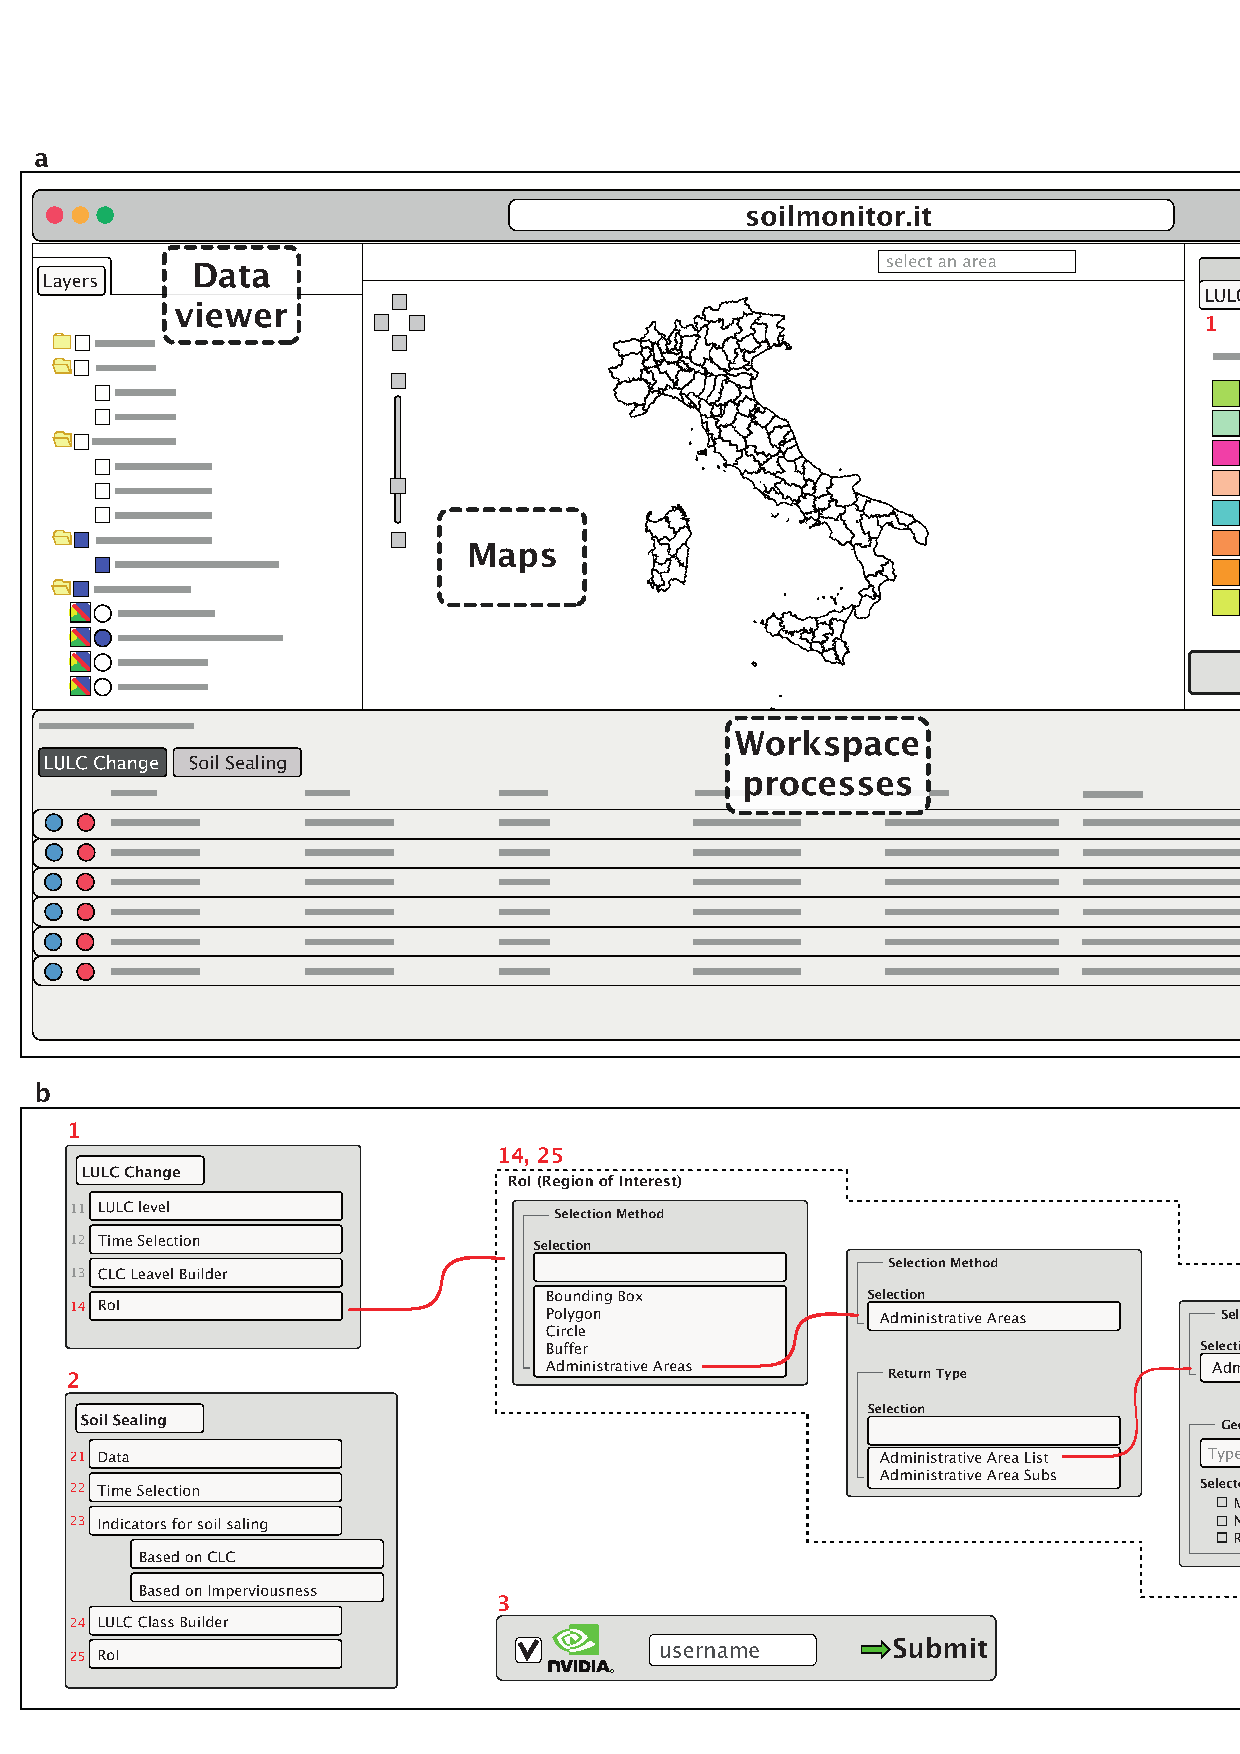
\includegraphics[width=500pt]{01_piattaforma.pdf}}
    \caption{Soil Monitor web application.
             (a) Exemplification of the dashboard with main panes (back dashed boxes), with reference to specific accordion panes (red annotations 1, 2, 3) described in (b). 
             (b) The user can build a tailored query owing to the job submission steps (section \ref{sec:jobsubmission}) thanks to two distinct accordion panes, one designed for the LULC change analysis (red 1) and another one dedicated to the soil sealing quantitative monitoring (red 2). A dedicated and advanced RoI building is available (red 14 and 25). Geospatial calculations can be distributed on GPU cards owing to a tailored CUDA-C library embedded in Soil Monitor (red 3).
             (LULC: Land Use and Land Cover; RoI: Region of Interest; CUDA: Compute Unified Device Architecture)
            } \label{fig:SMapp}
\end{figure}

Soil Monitor is based on a three-tier logical architecture (Figure\ref{fig:GCI}) with separated processes made by 
(i) 
the \textit{data tier} (section \ref{sec:dataTier}), which consists of the database where information is stored and retrieved in a manner that keeps data neutral and independent of the application servers and of the logic tier,
(ii) the \textit{visualization tier} (section \ref{sec:viewTier}), which displays information related to the data and services
and 
(iii) 
the \textit{logic tier} that controls the functionality of the application by performing detailed geospatial processing (section \ref{sec:logicTier}).

\begin{figure}[t] % FIGURE 02
    % \includegraphics[width,,height=15pc,draft]
    % trim=left bottom right top, trim=0 0 0 50,clip,
    \centerline{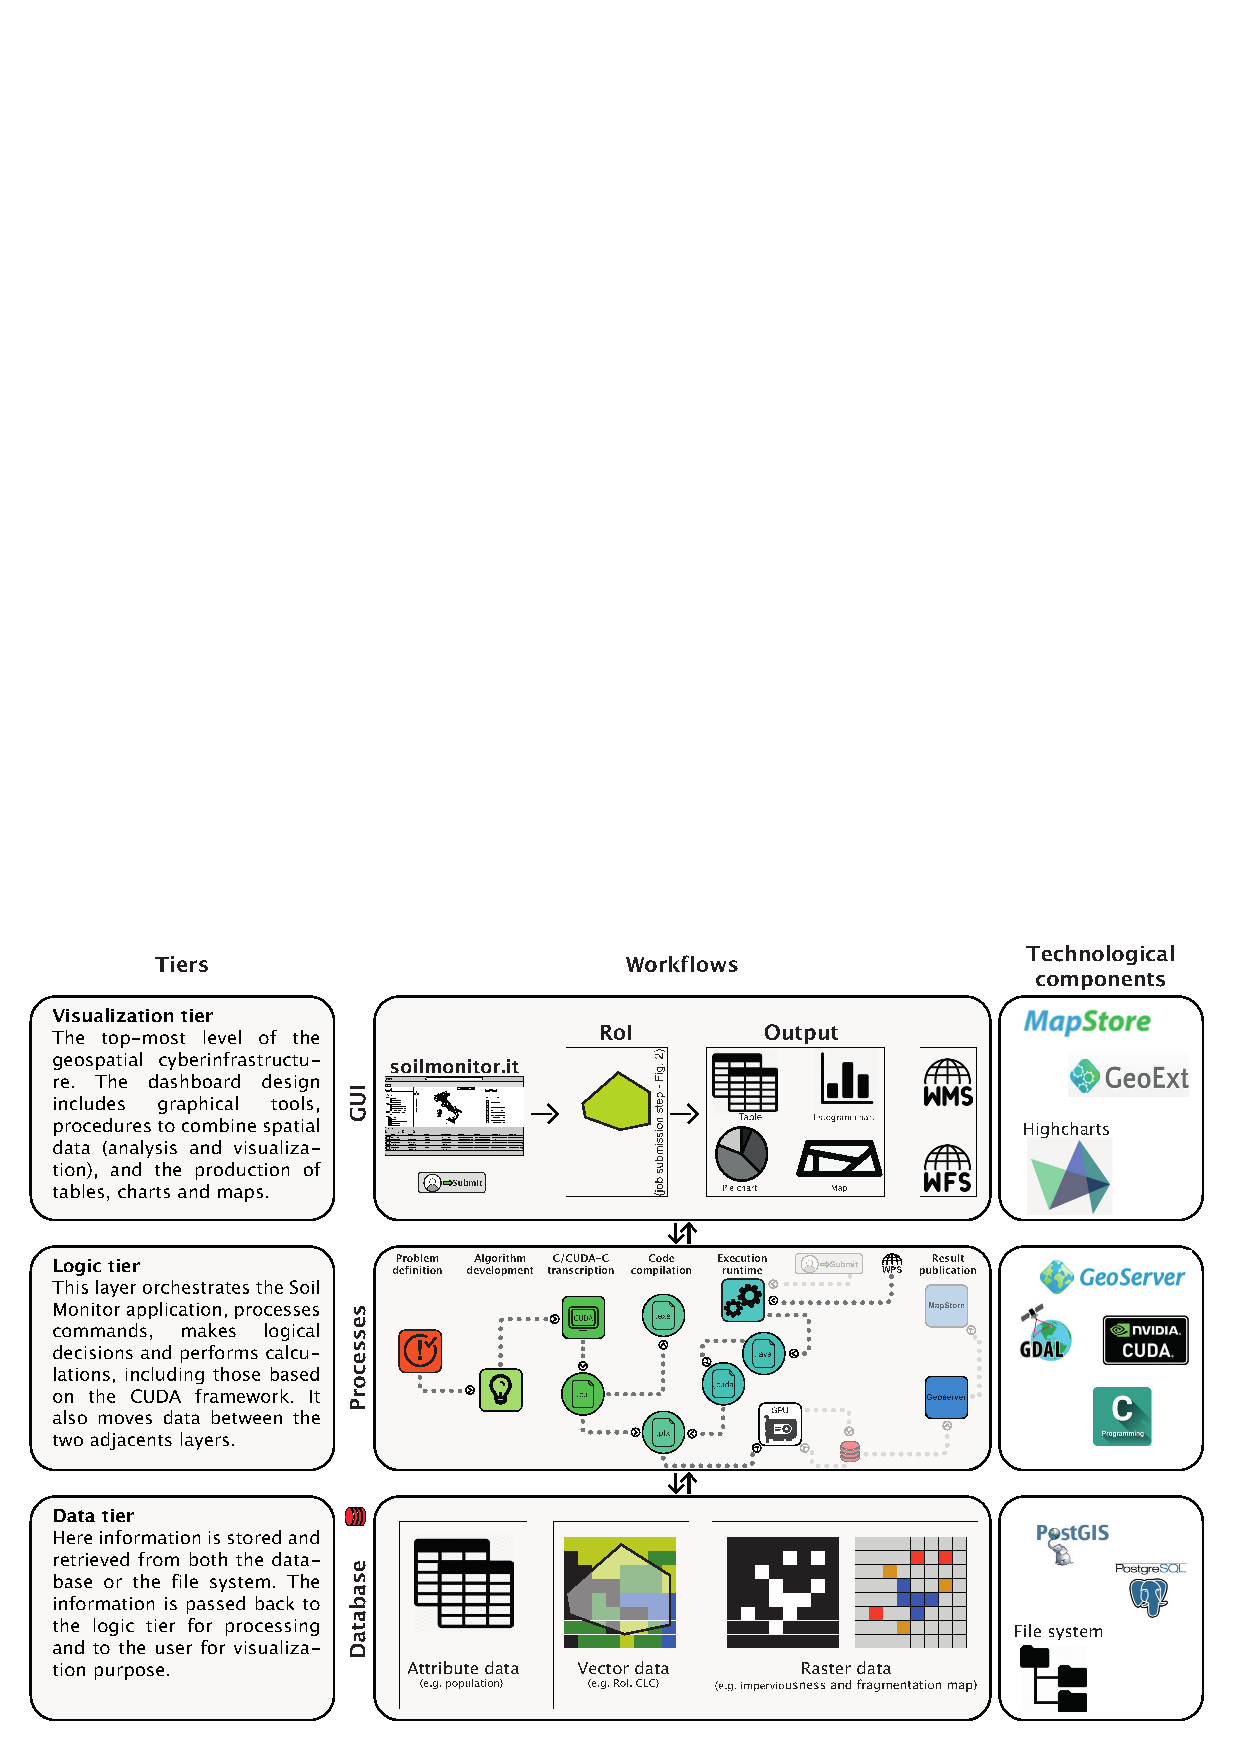
\includegraphics[width=500pt]{02_infrastruttura.pdf}}
    \caption{Main tiers, workflows, and technological components of the geospatial cyber-infrastructure behind Soil Monitor.
    The operating mode of the platform is sketched showing the flow of data that feeds different server functions (e.g. models), which, in turn, produces a set of services that can be finally accessed by the dashboard.
    (GUI: Graphical User Interface; RoI: Region of Interest)
    } \label{fig:GCI}
\end{figure}

%The data and visualization tiers are described in section \ref{sec:dataTier} and section \ref{sec:viewTier} respectively, while a summary of the logic tier is in section \ref{sec:logicTier}.


\subsection{Data (data tier) }
%\update{[materials]}}
\label{sec:dataTier}
The Open Geospatial Consortium, which aims to develop community-consensus open geospatial standards, provides a family of enabling technologies for sharing geospatial data and analytical capabilities on a distributed network. 
Data sharing (interoperability) in Soil Monitor is supported both in input --- to visualize data coming from remote services (e.g. those provided by ISPRA (Italian Institute for Environmental Protection and Research) or other national level administrative bodies) --- and in output to provide different data services such as WMS (Web Mapping Service, for serving georeferenced map images over the internet) and WFS (Web Feature Service, which supports the vector data model). % to allow a client visualization of output images produced by the logic tier.
These web services are automatically appended to the output images produced by the logic tier %new geospatial data %calculated by the CUDA engine 
to enable the visualization of results both locally within Soil Monitor, and remotely, for instance, within desktop GIS software environments.
Indeed, after ingestion in GeoServer, data become available for visualization and calculation purposes for the whole Italian territory Soil Monitor stores as follows:
\begin{itemize}
    \item The Land Use and Land Cover (LULC) map in the period of 1956-60 produced by the Italian Touring Club in collaboration with National Council of Research, CNR (map of land use in Italy, scale 1: 200.000).
    \item The CORINE Land Cover (CLC) is a valuable source of information about land use and land cover, produced at the European level since the '90s and updated regularly (originally coordinated by the European Commission and the European Environmental Agency; now included in the Copernicus framework).
    CLC vector data are produced by photointerpretation of satellite images, with a minimum mapping unit of 25 ha and a classification system organized in three hierarchical levels of thematic detail: level 1 with 5 land use and land cover classes, level 2 with 15 land use and land cover classes, and level 3 with 43 land use and land cover classes. 
    In Soil Monitor, the raster version of CLC with a spatial resolution of 100 m is available for the years 1990, 2000, 2006, 2012, and 2018. Considering the homogeneity over the entire Europe and the constant update, CLC is largely used for spatial analysis, land cover change assessment, and policy making.
    \item The National High-Resolution Soil Consumption (NHRSC) dataset was produced for Italy by ISPRA (ISPRA, 2016); the NHRSC is a raster that identifies artificial land cover areas with a spatial resolution of 10 m, produced for 2006, 2009, 2012, 2015, 2016, 2017 and 2018 with a semi-automatic classification of satellite images and the integration of local ancillary data such as OpenStreetMap; NHRSC included in Soil Monitor has a binary classification system such as non-sealed soil and sealed soil, according to the description given in Table \ref{tab:IMPclasses}.
    \item The administrative units: Italian administrative data are provided by the Italian institute of statistics (ISTAT). 
    These data represent the administrative units (also NUTS) in vector format.
    \item The population: population data are provided at the Municipal level by ISTAT, which periodically collects census data and updates this information every year. 
    \item The digital soil grids: Predictions on key soil properties performed globally at 250 m spatial resolution by ISRIC\footnote{available at http://data.isric.org/geoserver/sg250m/wms}. This is an example of Open Geospatial Consortium compliant interoperability based on WMS which is used as input source of georederenced map images in Soil Monitor.
\end{itemize}

\begin{table}
\caption{Legend and classes of the National High-Resolution Soil Consumption dataset}\label{tab:IMPclasses}
\centering
\begin{tabular}[t]{ l l | l } 
\hline
\textbf{Code} & \textbf{Description} & \textbf{Classes} \\
\hline
\multirow{9}{4em}{0} & \multirow{9}{10em}{Non-sealed soil} & Tree/shrubs \\ 
 &  & Crops \\ 
 &  & Grassland \\ 
 &  & Water bodies \\ 
 &  & Wetlands \\ 
 &  & Rocks, beaches, and dunes \\ 
 &  & Glaciers and perpetual snow \\ 
 &  & Sport areas (pervious surface) \\ 
 &  & Other pervious surfaces \\ 
\hline
\multirow{10}{4em}{1} & \multirow{10}{10em}{Sealed soil} & Buildings \\ 
 &  & Road/Squares/Parking \\ 
 &  & Railway sites \\ 
 &  & Airports and ports (impervious surfaces) \\ 
 &  & Impermeable areas in sports fields \\ 
 &  & Permanent greenhouses \\ 
 &  & Solar farms on land \\ 
 &  & Mining areas \\ 
 &  & Dump sites \\ 
 &  & Other impervious areas \\
\hline
2 & Unclassified & \\
\hline
3 & Area outside the national boundary & \\
\hline
\end{tabular}
\end{table}

The CLC and Touring layers have been rasterized into images at 8-bit and 100 meters resolution to enable the grid-based calculations. % based on the CUDA framework.
Comparisons between CLC layers can be executed at three different levels of the legend detail (Level 1, Level 2, and Level 3) having different numbers of land use and land cover classes. 
In order to enable comparisons with the Italian Touring Club layer, the most detailed CORINE legend (Level 3) has been homogenized with that from Touring Club. 
The imperviousness layers have been binarized (2-bit images) by applying a threshold to the level of imperviousness equal to 30\% of the pixel area, above which a pixel is taken as sealed.

\subsection{Development of the dashboard (visualization tier) }
%\update{[methods]}}
\label{sec:viewTier}
% Visualization of data and use of soil sealing tools
The dashboard design includes graphical tools, procedures to combine spatial data (analysis and visualization), and the production of tables and maps. 
The frontend application is based on MapStore (Figure \ref{fig:GCI}) and the overall structure of the graphical user interface can be distinguished in four main panes: the data, the map, the workspace, and the analysis panes (Figure \ref{fig:SMapp}a, dashed boxes).
The \textit{data pane} enables the visualization of different data, but not all information used in the calculation is visible, such as the population vector data. 
Moreover, MapStore enables users to add external data sources equipped with web services for rendering rasters and vectors, enhancing the overall interoperability of the platform. 
For instance, it can be particularly useful to compare the result of calculations with constraint maps coming from other data providers, such as the Italian Ministry of Cultural and Environmental Heritage, to check the soil sealing results. Furthermore, the \textit{map pane} enables the visualization of both the input geospatial data and the output maps calculated by the models and indicators available in the toolboxes. 
Moreover, the \textit{workspace pane} is where all instantiated requests are displayed. 
The toolboxes enable the allocation of several asynchronous requests per single user at the same time, which means that they can be calculated concurrently on the available CPU and GPU resources. 
The processes launched by users, which may be running at the same time, are displayed in the workspace as running, completed or interrupted according to their states. 
The \textit{analysis pane} is made by two dedicated \textit{accordion panes} (Figure \ref{fig:SMapp}b, red annotations 1 and 2) that are available to give the user full access to the logic tier parameters in a transparent way.

In addition to standard open-source codes available from the dual infrastructure GeoServer and MapStore, new codes have been written to enrich the functionality of Soil Monitor.
For example, the client side has a dedicated interface to build a customized RoI (more details provided in the job submission, section \ref{sec:jobsubmission}) and the availability of different types of Highcharts plots that are generated dynamically in addition to the visualization of map images, in order to enhance the readiness and interpretation of results.

\subsection{Soil sealing metrics embedded in Soil Monitor } %\update{[methods]}}
\label{sec:metrics}
Huge amount of metrics is available to monitor and measure urban growth, urban density and sprawl, soil sealing and land take.
The limited list of indicators developed and implemented in Soil Monitor have been chosen in close collaboration with italian urban planners to address their specific needs while avoiding redundancy of information often given by similar metrics. 
A summary of available metrics is given in Table \ref{tab:SMappToolbox}.
They include land use and land cover metrics, rate of change of land use and land cover, marginal soil sealing, extent of urban sprawl, density of urban boundaries, degree of urban dispersion, rural and urban fragmentation, land take dynamics, and estimate of loss in food supply due to land take. 

The metrics shown in Table \ref{tab:SMappToolbox} can use as input one of the two official datasets described in the data tier section above, that is a grid of LULC or a grid of soil imperviousness. 
The LULC layers allow investigations on multiple classes of land use and land cover but at a relatively coarser spatial resolution (either 100 m or 250 m spatial resolution with the CLC or Touring Club data, respectively).
Conversely, soil imperviousness is available over high spatial detailed layers (20 m spatial resolution) but aggregates the information of land use in only two classes, that is sealed and unsealed land as defined in Table \ref{tab:IMPclasses}. 
Finally, the choice between the two datasets reflects the kind of soil sealing metric, the detail in the thematic domain, and the spatial resolution required in the output map.

\begin{table}[b]
    \caption{ Metrics implemented in Soil Monitor for soil sealing and land take. }
    \label{tab:SMappToolbox}
    \small
    \centering
    \begin{tabular}{m{0.3cm} p{0.1cm} p{1.2cm} p{3.5cm} *{3}{p{2.7cm}} p{1.0cm} }
    
    \toprule
        & \textbf{ID} & \textbf{Model} & \textbf{Formula$^\dagger$} & \textbf{Description} & \textbf{Application} & \textbf{Techonological Novelty} & \textbf{Outputs}\\
    \midrule\midrule
    
    \multirow{5}{*}{ \rotatebox[origin=c]{90}{ \shortstack[c]{ Calculation using LULC rasters at 100m spatial resolution \\ (e.g. CLC produced by Copernicus)} } } 
    & 0 & LULC & --- & Change of state of each LULC class from a reference year to a current year & Evolutionary trajectories & CUDA kernels producing both an interactive change matrix and a map of all changes & pie chart, raster map  \\
    
    & 1	& Coverage Coefficient & $\frac{S_{CLC_i}}{S_{AU}}$ & Fraction of total surface covered by i-th land use/cover class & Classes consistency within a user defined RoI (admin unit or free area) & None & bar chart, vector map \\
        
    & 2 & Rate of Change & 
    $\frac{ \left(S_{CLC_i}\right)_{T_2} - \left(S_{CLC_i}\right)_{T_1} }{ \left(S_{CLC_i}\right)_{T_1} }$ 
    & Rate of change of any i-th land use/cover class & Change of classes consistency within a user defined RoI (admin unit or free area) & None & bar chart, vector map \\
    
    & 3 & Marginal Land Take & 
    $\frac{ \left(S_{CLC_1}\right)_{T_2} - \left(S_{CLC_1}\right)_{T_1} }{ \left(POP_{au}\right)_{T_2} - \left(POP_{au}\right)_{T_1} }$
    & Ratio between urbanization variation and population growth variation between two years & Analyse variation of urbanization with respect to variation of population to depict temporal trends & None & bar chart, vector map \\
    
    & 4	& Urban Sprawl & 
    $\frac{ \frac{ \left(S_{CLC_1}\right)_{T_2} - \left(S_{CLC_1}\right)_{T_1} }{ \left(S_{CLC_1}\right)_{T_1} }  }     { \frac{ \left(POP_{au}\right)_{T_2} - \left(POP_{au}\right)_{T_1} }{ \left(POP_{au}\right)_{T_1} } }$
    & Ratio between urbanization rate and population growth rate between two years & Standardized version of marginal land take & None & bar chart, vector map \\
    
    \midrule
    
    \multirow{9}{*}{ \rotatebox[origin=c]{90}{ \shortstack[c]{Calculation using high resolution imperviousness rasters at 20m spatial resolution \\ (NHRSC produced by ISPRA)} } } 
    & 5 & Urban sprawl & 
    $\frac{S_{DUF}}{S_{UT}}$ 
    & Ratio between discontinuous urban fabric and total urban surface & To know the composition of urban development related to sprawl phenomenon, which can be related to fragmentation & Tailored connected component labelling algorithm in CUDA & bar chart \\
    
    & 6 & Edge Density (ED) &
    $\frac{P_{UT}}{S_{UT}}$ 
    & Ratio between perimeter and surface of urbanized ares in selected RoI & Density of urban margins, which is related to urban fragmentation & CUDA kernels computing both the perimeter and the urbanized area & bar chart \\
    
    & 7 & Urban Area &
    $\frac{S_{UT}}{S_{AU}}$ 
    & Fraction of total surface covered by urbanization & To know the magnitude of land take related to the administrative unit & CUDA kernels computing the urbanized area	& bar chart \\
    
    & 8	& Largest Class Patch Index (LCPI) & 
    $\frac{S_{max}}{S_{UT}}$ 
    & Fraction of urban surface within the largest urban patch & Represents the level of compactness of the urban area & CUDA kernels computing the connected component labelling	& bar chart \\
    
    & 9	& Residual Mean Patch Surface (RMPS) &
    $\frac{S_{DUF}}{N_{DUF}}$ 
    & Average surface of all urban patches excluding the largest patch & Mean patch area within the discontinuous urban fabric, which can be related to urban texture & CUDA kernels computing the connected component labelling & bar chart \\
    
    & 10 & Rural/Urban Fragmentation &
    $\frac{\sum^{N}_{k=1} V_k}{ N-1 }$ 
    & Fraction of pixels having the same value of the centre pixel in a mask & e.g. on rural centre pixels it highlights ecological corridors & 1k lines of code; 6 CUDA kernels; 8 geospatial parameters & raster map \\
    
    & 11 & Land Take (and Gains) &
    $ \left( V_{pix} \right)_{T_2} - \left( V_{pix} \right)_{T_1}$ 
    & Difference of the value of a pixel between two different times & A map with three possible pixel values: (0) if no change occurred; (-1) if land take; (+1) if land gain & Based on the basic reduce CUDA kernel & raster map, bar chart \\
    
    & 12 & Net Loss of Food Supply &
    $ \sum_{pix=0}^{image} \left( \left( V_{pix} \right)_{T_2} - \left( V_{pix} \right)_{T_1} \right) \times C $ 
    & --- & Potential loss of aggregated ecosystem function (coeff :: FAO) & Based on the basic reduce CUDA kernel & bar chart \\
    
    & 13 & Model of Urban Development & Composite of IDs 6, 8 and 9 & --- & ---	& Same as aggregating IDs 6, 8 and 9 plus a 3-D view highlighting urban development in both different administrative units and times & 3-D scatter plot \\
    
    \midrule\bottomrule
    
    \multicolumn{8}{p{17.2cm}} % 13.9cm is the sum of all column previously defined by p{}
    {
      \footnotesize{$^\dagger$Definitions. 
      $S$:area;
      $P$:perimeter;
      $V$:value;
      $S_{CLC_i}$:area of $i_{th}$ CORINE Land Cover class at selected legend level; 
      $S_{AU}$: area of administrative unit; 
      $S_{CLC_1}$: area of urban CLC class at selected legend level; 
      AU: administrative unit (city, province, region, \ldots); 
      $T_1$: time before; 
      $T_2$: time after; 
      $POP_{AU}$: population within AU; 
      $S_{DUF}$: area of discontinuous urban fabric; 
      $N_{DUF}$: number of urban patches within discontinuous urban fabric; 
      $S_{UT}$: total urban area; 
      $V_k$: amount of fragmentation of the target pixel \textit{k} within the moving window of N pixels };
      $V_{pix}$:value of pixel in NHRSC raster;
      C: FAO coefficient equal to 0.6 $persons \times ha^{-1} \times year^{-1}$
      .
    }
    \end{tabular}
\end{table}

\subsubsection{ Soil sealing metrics operational: the fast geoprocessing engine (logic tier) } % \update{[methods]} }
\label{sec:logicTier}
%\update{We need a description of the logic tier avoiding it being viewed as a technical report/manual}\\
On the server side, specific functions written in Java (classes) and CUDA (kernels) have been developed to perform the calculations required by the metrics reported in Table \ref{tab:SMappToolbox}. 
Some calculations may be very demanding since they rely on high resolution grids (i.e. a square pixel of size 20 m) or on high thematic detail (i.e. CORINE land cover at level 3 with 43 classes) feeding requests over large geographical areas (such as administrative regions or the whole Italy).
These cases may not manage to return answers in real-time or near-real-time
%for relatively large geographical extents
, which explains why 
(i) calculations are instantiated asynchronously in the geospatial cyber-infrastructure, and
(ii) metrics are implemented in GPU computing using the CUDA framework by NVIDIA.
The asynchronous instantiation of calculations in the cyber-infrastructure means that a a request can be submitted without waiting for previous ones to be finished.
This allows both the multi-user concurrency and the submission of as many requests as needed by a single user to address own analysis.
The user can close the web page and then navigate back to the Soil Monitor workspace to find the results ready for visualization and interpretation.

The second characteristic of the geoprocessing engine is the implementation of most of the metrics showed in Table \ref{tab:SMappToolbox} by means of the CUDA-C programming language.
The CUDA code and its binding from Java is implemented in the logic tier in which %is connected to the data tier and the visualization tier.
%In the logic tier a 
the list of developed CUDA kernels is loaded as a library in the infrastructure.
The development of the fast geoprocessing engine is as follows (see the workflow in logic tier of Figure \ref{fig:GCI}).
First, a library of CUDA kernels is written in C and then compiled in PTX. 
Second, the most fundamental CUDA kernels work as primitives that are assembled in the JCUDA layer to build the crafted algorithms  addressing the calculation of soil sealing metrics.
This is referenced as the Java/JCUDA/CUDA pipeline of Soil Monitor.% which is a novelty in the implementation of spatial decision support systems using WebGIS over the internet.

In addition to data services (section \ref{sec:dataTier}), Soil Monitor implements Web Processing Services (WPS) which expose algorithm of soil sealing metrics outside the web application (Figure \ref{fig:GCI}, logic tier). 
WPS allows to invoke a geospatial process with a known set of parameters by means of the supported POST request method (using the XML language) submitted directly to the GeoServer endpoint (JAVA layer).
After the submission of the request using either the Soil Monitor graphical interface or the POST method, the parameters are passed to the JCUDA layer, which, as a software bridge, invokes the execution of the CUDA kernels compiled in PTX files.
This is recognized as the \textit{forward} high performance computing phase of the geoprocessing engine, which spans from the request submission step by the user to the matrices production in CUDA.
The matrices returned after CUDA calculations are manipulated to become GIS data that are stored in GeoServer.
This is the \textit{backward} geoprocessing phase of the engine, which spans from the production of CUDA matrices to the storage of map images in a WebGIS environment.
Finally, the map images can be visualised over the Soil Monitor web application (see the visualization tier in section \ref{sec:viewTier}).


\subsection{Job submission: how to run metrics and perform quantitative analysis}
\label{sec:jobsubmission}
It was required to implement a systematic workflow approach in the cyber-infrastructure in order to integrate the fast geoprocessing engine based on CUDA kernels with both data and open source geospatial components given by GeoServer (backend) and MapStore (frontend). 
The systematic workflow implemented in Soil Monitor is designed around the end user and includes three major consecutive steps: job submission, the query of job status (e.g. running, completed, failed), and the management of results.
The execution of each step requires a close integration of the three software tiers in the cyber-infrastructure, that is a strong connection between the data, visualization and logic tiers. 

Figure \ref{fig:SMapp} shows an overview of the available toolboxes for analysis, that is the toolbox for land use/cover change (Figure \ref{fig:SMapp}, red annotation 1) and the toolbox for soil sealing (Figure \ref{fig:SMapp}, red annotation 2).
The user can build a tailored query owing to a job submission step, one for each toolbox, separately. 
For any soil sealing metric, for instance, the user must select --- according to the following hierarchical order --- 
the dataset they intend to use (i.e. land use/cover or high-resolution imperviousness, Figure \ref{fig:SMapp}, panel b, red annotation 21); 
the time of the analysis (one year or two years, Figure \ref{fig:SMapp}, panel b, 22); 
the selection of a soil sealing indicator (Figure \ref{fig:SMapp}, panel b, 23); 
optionally, the composition of LULC classes (Figure \ref{fig:SMapp}, panel b, 24); 
finally, the region of interest (Figure \ref{fig:SMapp}, panel b, 25). 
To ease the definition of a possible multi-polygon RoI, there is an ad hoc accordion pane for the rapid identification and selection of any Italian administrative unit.
The RoI accordion pane is particularly useful because in addition to freely draw a new region of interest directly over the map, the user can either manually add the administrative units at any level of the topological hierarchy (municipality, province, region) 
or automatically add all the administrative units belonging to an administrative unit of the level above (i.e. all the municipalities belonging to a selected province) as carried out in the quantitative analysis at the municipality level (section \ref{sec:caseCOM}).

For any subsequent query to the first one, the user can change only the parameters strictly required for the new job submission (e.g. change only the indicator used or the time of the analysis) and Soil Monitor will calculate the new indicator given the parameter set just defined. 
This behaviour was expressly required by end users to facilitate the instantiation of more requests for the purpose of scrutinizing the implementation of executed urban plans.
Two job submission examples are provided in the following sections highlighting some technical details about their implementation.

\subsubsection{Calculate the map of rural fragmentation}
\label{sec:mmFragmentation}
The fragmentation metric is computed on binary imperviousness layers with 20 m spatial resolution and Soil Monitor manages both rural and urban fragmentation.
Fragmentation quantifies how much fragmented % (or conversely, the degree of integrity) 
a target pixel in the center of a moving window is (Table \ref{tab:SMappToolbox}, $ID = 10$).
Besides other filters such as time and RoI, the job submission for fragmentation requires to configure the size of the moving window (e.g. 800 m) and the type of fragmentation (rural or urban).
In the case of rural fragmentation, the target is a non-sealed pixel with value 0 (assumed to be not sealed at all or covered by impervious materials on a maximum of 30\% of the total pixel area) and all sealed pixels (with value 1) within the moving window are summed to calculate the $V_k$ of the fragmentation formula reported in Table \ref{tab:SMappToolbox}.
Contrariwise, in urban fragmentation the target pixel has value 1 and not-sealed pixels (with value 0) are counted.
The calculation of fragmentation relies on inherently demanding geospatial processing.
Indeed, even if selecting a small RoI, the relatively high calculation demand depends on the logic of the algorithm itself, since it has to visit about six thousand neighbour pixels $\left( \sim \left( \left(800/20\right)\times2 \right)^2 \right)$ to calculate how fragmented each target pixel is, given a radius of 800 meters in the moving window selected by the user.

\subsubsection{ Calculate the discontinuous urban fabric surface }
\label{sec:mmDUF}
The discontinuous urban fabric surface ($S_{DUF}$) is calculated by Soil Monitor in the backend and the user cannot directly manage it (no dedicated job submission). %, hence there is any job submission to get this directly this result.
The implementation is challenging because it is required (i) to perform real-time calculations using (ii) the National High-Resolution Soil Consumption dataset as input.
To address these requirements, a connected component labelling algorithm specifically developed for Soil Monitor was implemented in CUDA.
Connected component labeling is a basic algorithm in image processing and an essential step in nearly every application dealing with object detection.
It is made of eight CUDA kernels and about one thousand lines of code, thanks to which the algorithm groups together pixels belonging to the same connected component (e.g. object).
Therefore, in our case it performs the labelling of the 2-bit imperviousness layer into a 64-bit layer of ordered and unique labels, one for each distinct urban patch (i.e. object).
The discontinuous urban fabric is assigned to areas generally lower than 25 ha in which artificially surfaced areas are associated with vegetated areas and bare soil.
For this reason after identification and labelling, urban patches are sorted and then a threshold (e.g. 90\%) is applied to extract only patches below the selected threshold (i.e. belonging to the discontinuous urban fabric).
These patches are summed to calculate the overall discontinuous urban fabric surface ($S_{DUF})$.
The results of this implementation are showed in section \ref{sec:resFRAG_DUF} according to the calculation of three different metrics.


\section{Validation of geoprocessing engine}\label{sec:validation}
During the implementation of the 
%Soil Monitor 
cyber-infrastructure we carried out a systematic testing procedure by means of web processing services as explained in section \ref{sec:logicTier}.
The WPS inferface was used to test and validate the fast geoprocessing engine because we could run from hundreds to thousands times calculations without the tedious infilling of the accordion panes over the graphical user interface to submit more and more requests.
POST requests are generally submitted from within the Unix terminal but for validation purpose they were submitted from within MatLab scripts. %, which were specifically designed to validate the geoprocessing engine.
To validate each Soil Monitor model, we collected and compared the results returned by the following three independent computing environments:
\begin{itemize}
    \item Running the stand-alone executable (EXE) compiled from the source CUDA-C code (Figure \ref{fig:GCI} logic tier).
    The source high performance computing code written in CUDA-C can be compiled to get either a stand-alone executable (EXE) or the executable file (PTX) embedded in Soil Monitor.
    In this step we run the stand alone executable passing as input the same data and parameters used in the other computing environments.
    This computing environment is used to validate the goodness of the high performance computing algorithm implemented in CUDA-C.
    \item Running the WPS as explained above.
    It is based on the Java/JCUDA/CUDA chain which executes the CUDA kernels compiled in the PTX files. This computing environment is crucial to validate together the forward high performance computing step and the backward geoprocessing step embedded in the geospatial cyber-infrastructure of Soil Monitor (see section \ref{sec:logicTier} for the two steps). 
    \item Running a MatLab code which implements the same geospatial processing but with a different algorithm.
\end{itemize}

The validation ends after a comparison of results coming from the three environments which enables to check for both speed performance and accuracy. 
This procedure was used as a standard during the development stage in order to test for inaccuracies in either the CUDA algorithms targeted to geospatial processing or in the deployment of the Java/JCUDA/CUDA computing chains in the cyber-infrastructure.

\section{ Results and Discussion } % \toberevised{Results} | remove or describe the fragmentation and DUF} }
\label{sec:results}

\subsection{ Fragmentation and discontinuous urban fabric surface }
\label{sec:resFRAG_DUF}
The calculation of both the fragmentation and the discontinuous urban fabric surface are examples of how powerful the implementations available in the geospatial cyber-infrastructure are.
A detailed explanation about how the calculation of the map of rural fragmentation is performed can be found in section \ref{sec:mmFragmentation}, while results are shown
 together with discussion
in the quantitative analysis provided at the province level (section \ref{sec:casePROV}).% to avoid verbosity.

Here the results of the implementation of the discontinuous urban fabric surface ($S_{DUF}$, Figure \ref{fig:ccl}) is provided as an example of the pyramidal architecture based on the CUDA kernels (i.e. as an example of the Java/JCUDA/CUDA pipeline).
The discontinuous urban fabric surface is calculated if the user requests the urban sprawl (Table \ref{tab:SMappToolbox}, $ID = 5$) or the residual mean patch surface (Table \ref{tab:SMappToolbox}, $ID = 9$) metrics.
Apparently, the calculation of these two indicators is very simple since they are computed as the ratio between 
% the discontinuous urban fabric surface 
$S_{DUF}$ and either the total urban area ( $S_{UT}$ in urban sprawl) or the number of urban patches within discontinuous urban fabric ($N_{DUF}$ in RMPS).
However, as demonstrated in section \ref{sec:mmDUF}, ten CUDA kernels are used to uniquely label each urban patch and then determine the number of pixels within it.
%its consistency in terms of the number of adjacent pixels within each patch.
This is one of the most powerful implementations available in the infrastructure, as a very small elapsed time (3.7 seconds) is required to complete the calculation over a very large region of interest (10000 x 18000 pixels, with 20m pixel size).
The $S_{DUF}$ is the final outcome depicted in figure \ref{fig:ccl} and is used to calculate the two metrics urban sprawl and RMPS.
As a final remark, it is highlighted the advantage of having a library of CUDA kernels implemented in Soil Monitor, which can be reused to easily calculate a new metric.
Indeed, the procedure till the sort of patches by size can be used to calculate the surface of the largest urban patch ($S_{max}$), which is used to quantify the largest class patch index (Table \ref{tab:SMappToolbox}, ID=8).

\begin{figure}[t] % FIGURE 03
    \centerline{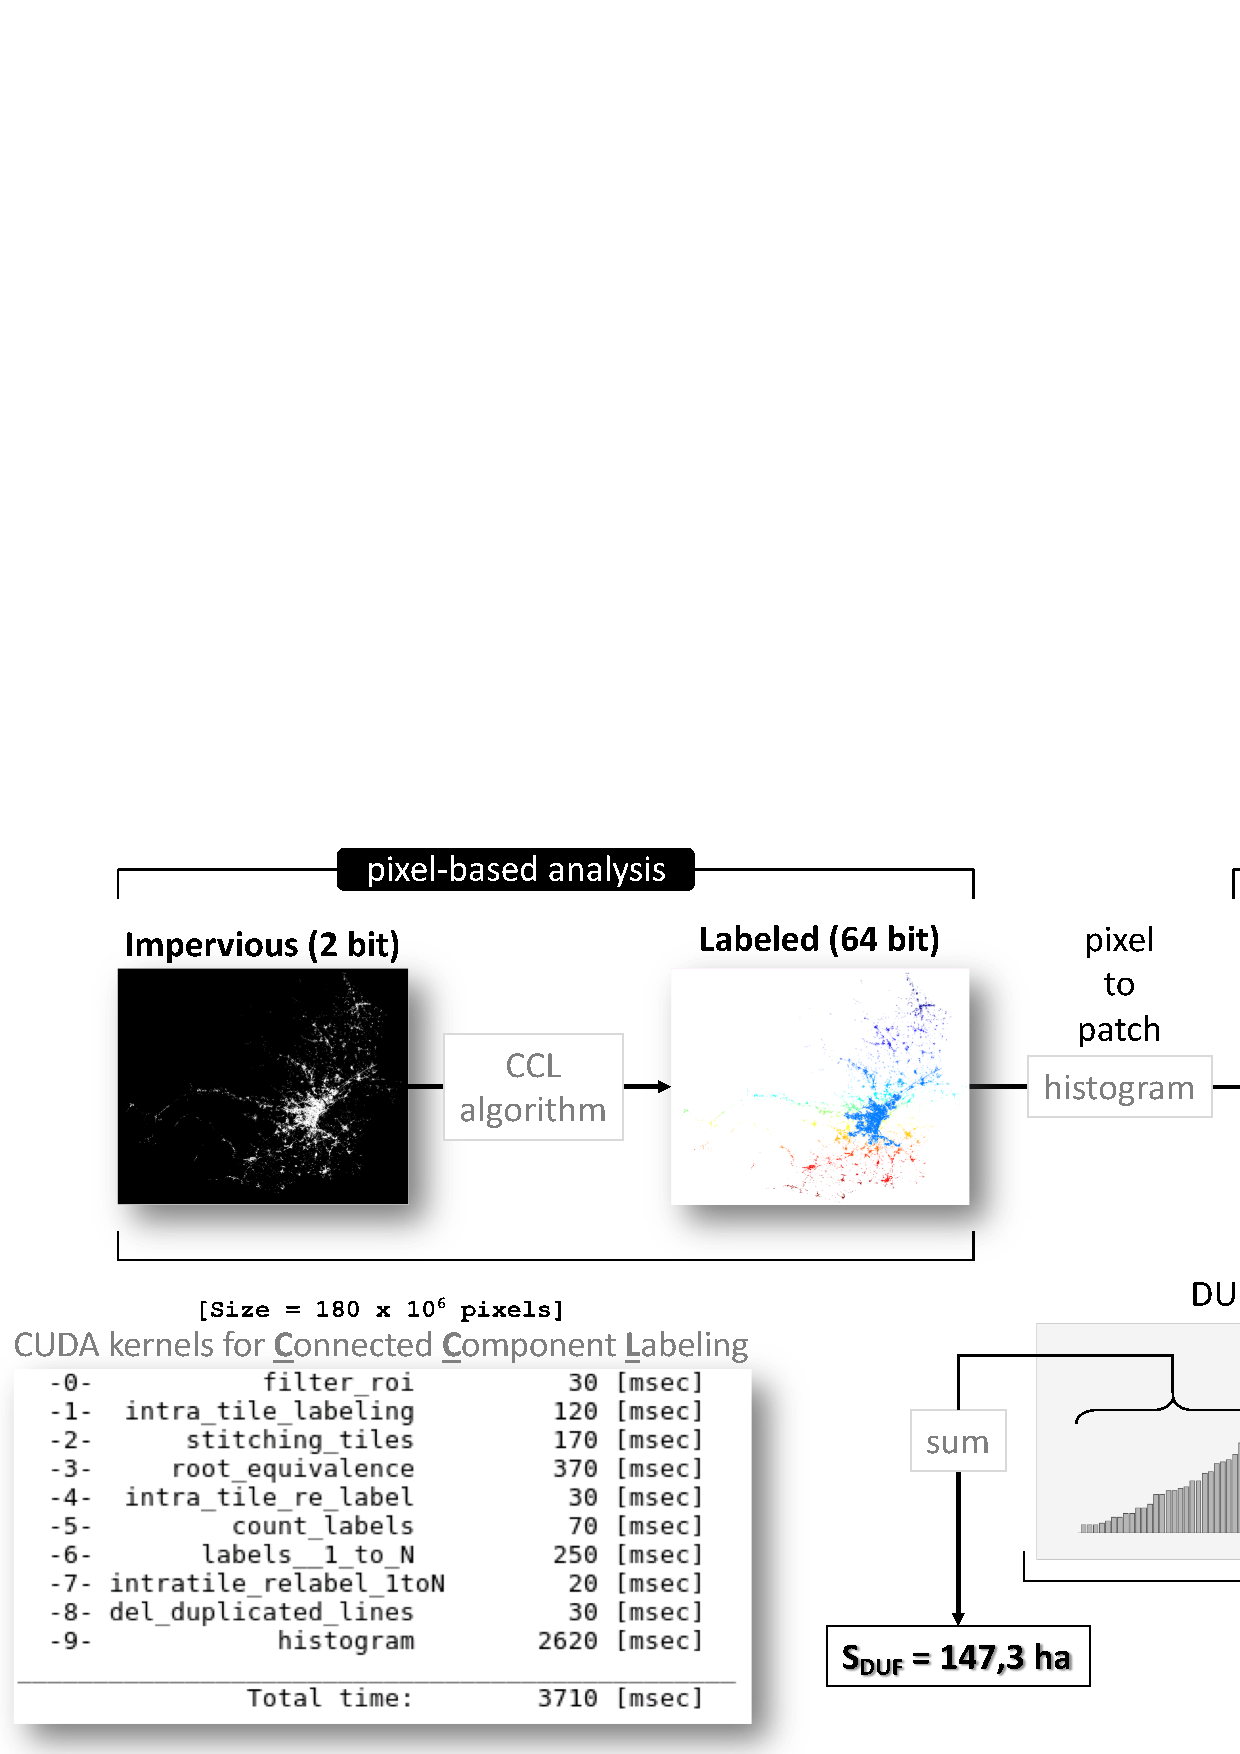
\includegraphics[width=500pt]{03_DUF_explanation.pdf}}
    \caption{ The calculation of the discontinuous urban fabric surface ($S_{DUF}$) developed within Soil Monitor cyber-infrastructure. 
    The pixel-based calculations are perfomed on the GPU card running a connected component labelling algorithm written in CUDA-C. 
    The patch-based calculations are performed on the CPU by Java code.
    The elapsed times in the box of CUDA kernels refer to an image of size $180 \times 10^6$ pixels using a NVIDIA TESLA C2075 GPU card.
    ( DUF = discontinuous urban fabric; CUF = continuous urban fabric; $S_{max}$ = largest urban patch surface)} \label{fig:ccl}
\end{figure}


\subsection{Quantitative monitoring and analysis on three Italian case studies using Soil Monitor}\label{sec:caseStudies}

\subsubsection{ Land use/cover monitoring for whole Italy } \label{sec:caseIT}
Land use/cover pattern is the consequence of natural and socio-economic factors and their utilization by man in time and space.
Knowledge about land use/cover, for instance assisted by monitoring, and potentialities for optimal use are crucial for the selection, planning and implementation of land use schemes that meet both the increasing demands for basic human needs and %welfare.
the changing demands of increasing population.
Consequently, accurate monitoring of the temporal changes of the land surface state is important to understand the relationship between man and nature and to provide decision makers with relevant information.
The information on vegetation change is probably the most important of these relationships and will be used in the following analysis.
The type and evolution of vegetation cover can be a powerful indicator of the magnitude of land degradation that is assessed by comparing land use/cover maps over different times.
Although land cover reflects the physical characteristics of earth's surface and differently land use refers to the way in which land has been used by humans, it is not possible to keep them separated in the following analysis.

In Italy, the monitoring of land take is accounted for by the National System for the Protection of the Environment (SNPA) as established by the entry into force of law 132/2016.
Accordingly, the SNPA is coordinated by ISPRA and involves all Italian Environmental Protection Agencies working at the regional level. 
This monitoring is scheduled in order to have an annually updated picture of the soil sealing evolution (e.g. ISPRA 2016, 2018) and the dynamics of land transformation and urban development, which is done through the production of thematic maps and the development of specific indicators. 
Law 132/2016 states that the SNPA must ensure such monitoring through monitoring points/networks or earth observation techniques (e.g. Copernicus).
In performing such monitoring, ISPRA and SNPA face two major problems: (i) difficult interaction with over 8000 Italian municipalities and (ii) the lack of awareness by citizens and other public authorities about the impact of soil sealing on land degradation.

In this framework, Soil Monitor can indeed represent an important step forward in land use/cover quantitative monitoring and analysis.
To show the results in Figure \ref{fig:caseIT}, the calculation of the matrix of land use/cover change was submitted to the platform using the whole Italy as RoI,
Touring and CLC as basic data and
the two contrasting yeas 1954 and 2012 as time filters.
The system produced an interactive change matrix with the land use changes between 13 different classes for the entire country.
From these data (see Figure \ref{fig:caseIT}\textit{a} and \textit{b}) it is very interesting to emphasise that the land use class mostly affected by new \textit{artificial surfaces} is the \textit{complex cultivation patterns} with a loss of 418,604 ha, that is the 26.72\% of transformation into \textit{artificial surfaces} in whole Italy from 50's to 2012 was possible due to the consumption of \textit{complex cultivation patterns}.
Since the matrix of changes generated by Soil Monitor is interactive, the click on the column of artificial surfaces produced either a pie chart (not shown) enabling an immediate and intuitive quantification of the changes by classes contributing to \textit{artificial surfaces} or an image map where it is possible to see where these changes have occurred (see the zoom of such a map in Figure \ref{fig:caseIT}\textit{c}).
It is possible to observe that the largest changes from \textit{complex cultivation patterns} to \textit{artificial surfaces} occurred at the fringes of earlier urban centres.


\begin{figure}[t] % FIGURE 04
    \centerline{\includegraphics[width=450pt]{04_caso_nazionale.pdf}}
    \caption{ The interactive change matrix calculation for whole Italy between 1954 and 2012.
    (a) The matrix of changes in hectares (ha) with particular focus on the column of \textit{artificial surfaces} (year 2012) with contributions coming from other classes (year 1954).
    (b) Same matrix of change as in (a) but expressed in percentage of the overall Italian area (except in parenthesis where percentages refer to the total of the class in header).
    (c) Map of \textit{artificial surfaces} (year 2012) with contributions coming from other classes (year 1954).
    } \label{fig:caseIT}
\end{figure}

\textit{Forests} covers one third (33.66\%) of the Italian area on 2012 and is one of the most conservative classes with respect to land take, since it only contributed by 4.41\% to the overall transformation into \textit{artificial surfaces} (the 0.23\% of total area).
Considering the above evidences along with the analysis of other land use classes, as a concluding remark the classes characterised by a lower level of specialization are the most fragile with respect to new land take.
\textit{Complex cultivation patters} and \textit{non-irrigated arable land} have suffered a tremendous general trade off with different other classes, because only about a quarter and half of their surfaces, respectively, remained unchanged between 1954 and 2012.
It quantifies the great impact of man pressure in solely 60 years, considering that \textit{complex cultivation patters} and \textit{non-irrigated arable land} together cover about the 42\% of the Italian territory.
On the contrary instead, classes such as \textit{vineyards}, \textit{olive groves} and \textit{fruit trees and berry plantations} are better defending, in particular against the land take aggression.
Therefore, higher specialization in agriculture would perhaps produce more resilient land use/cover classes to challenge new land take pressures.

By means of the Soil Monitor platform, we analysed the changes between 1954 and 2012 in further detail
for each separate Italian administrative region, with particular emphasis on quantifying changes in \textit{artificial surfaces}, \textit{forests} and \textit{complex cultivation patterns} (see Figure \ref{fig:caseIT_graphs}a).
Those regions, such as Lombardia and Veneto, experiencing a large land take (about 10\% and 8\% of their regional areas, respectively) are also most affected by a loss in \textit{complex cultivation patterns}.
On the contrary, regions affected by weak land take dynamics, such as Molise, Valle D'Aosta and Liguria show a better preservation of the \textit{complex cultivation patterns} class.

\begin{figure}
    \centerline{ 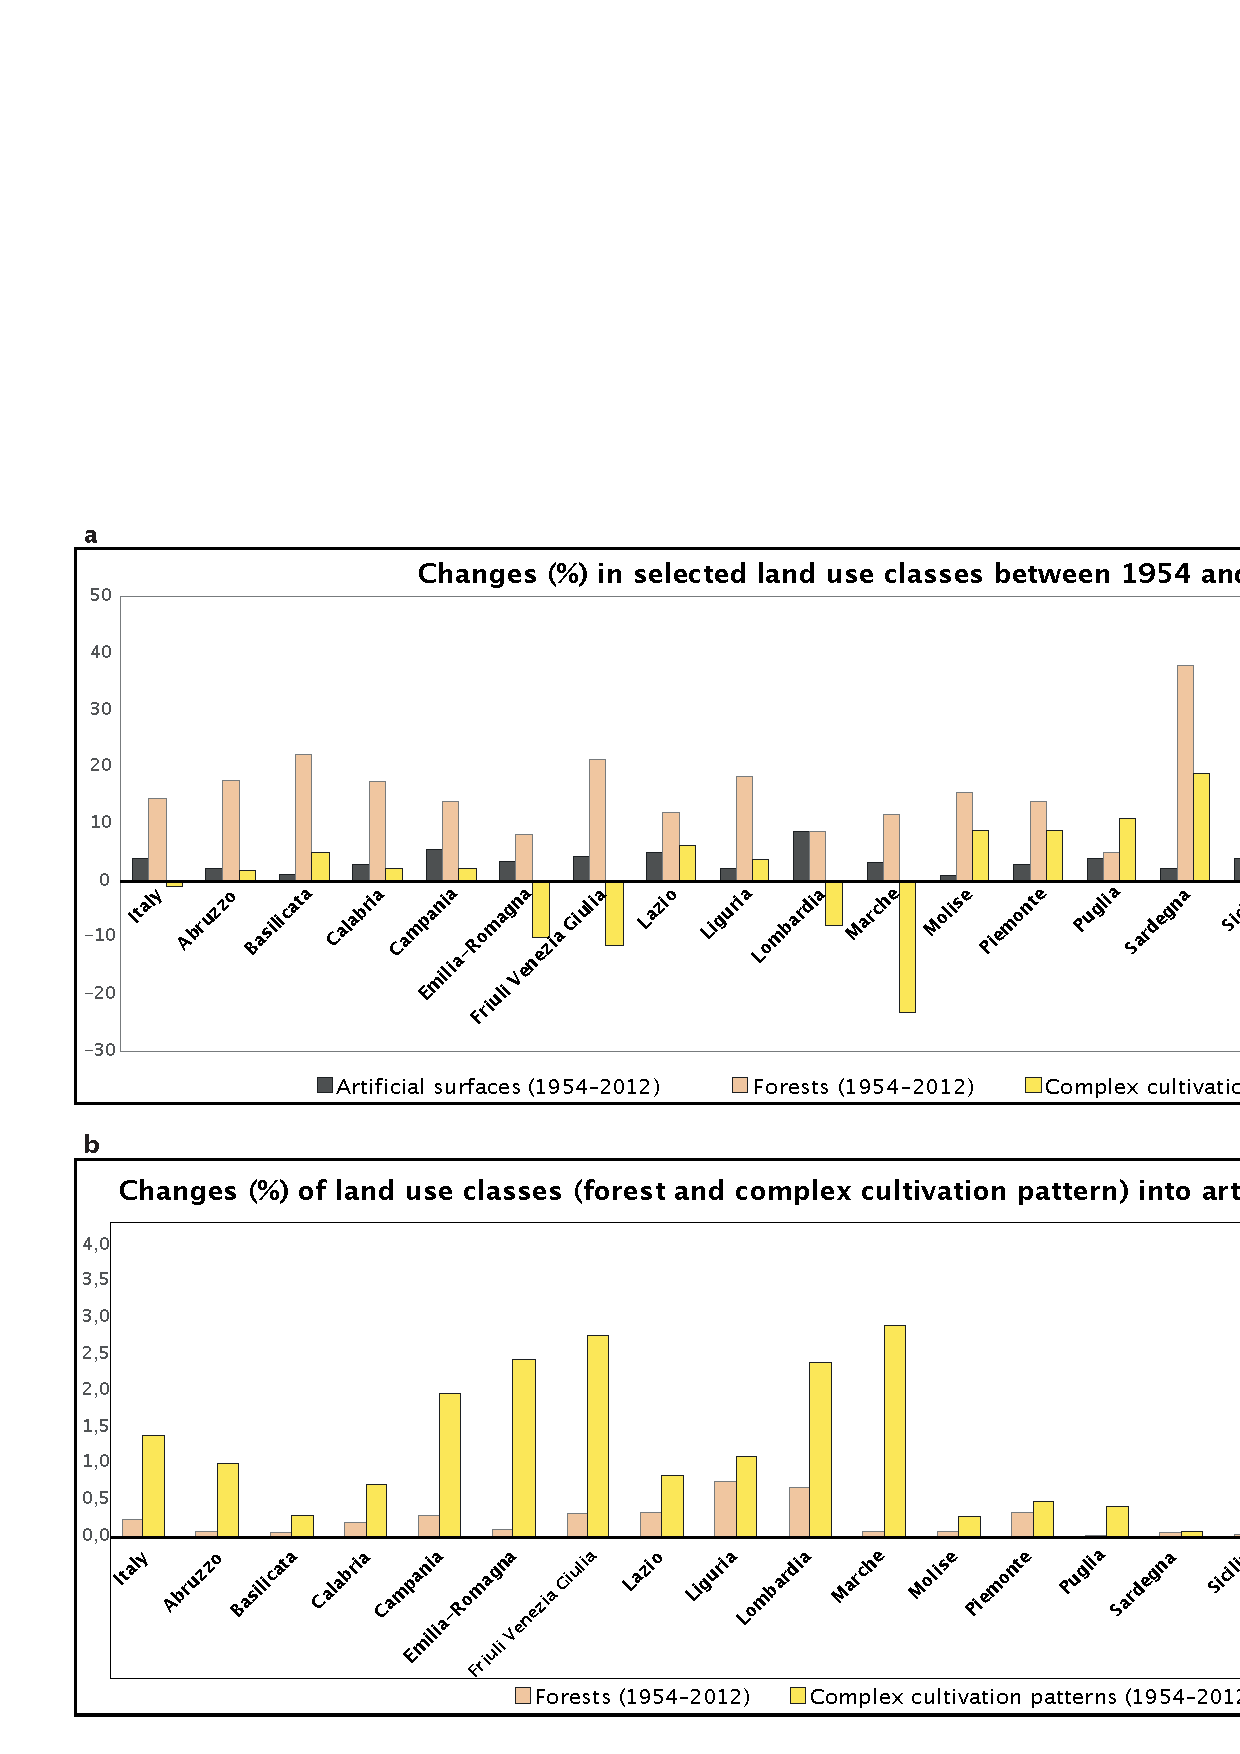
\includegraphics[width=450pt]{05_caso_nazionale_grafici.pdf} }
    \caption{Breakdown of changes between 1954 and 2012 by region assuming the regional area as total within each region.
             (a) Impact of regional changes on \textit{artificial surfaces}, \textit{forests} and \textit{complex cultivation patterns}.
             (b) Regional changes in the trade off between \textit{forests} and \textit{complex cultivation patterns} with \textit{artificial surfaces}.}
    \label{fig:caseIT_graphs}
\end{figure}

A close-up of the above evidences is reported in Figure \ref{fig:caseIT_graphs}(b) where we quantified the impact of artificial surfaces over \textit{forest} and \textit{complex cultivation patterns}. 
The areas covered by \textit{complex cultivation patterns} have been strongly challenged by land take in regions such as Veneto, Lombardia, Emilia Romagna and Friuli Venezia Giulia which have also the largest gross domestic production in Italy.


\subsubsection{The territorial plan at the province level (PTCP)}
\label{sec:casePROV}
In Italy, the reference administrative level for urban planning coordination in terms of environmental issues is the province law 142/1990. 
Thus, it is the key geographical level to challenge land take. 
However, this situation somehow remained unchanged after law 56/2014 (rules on metropolitan cities) and even after the constitutional referendum that transfers the competences of the provinces to the regions (4 December 2016).
Currently, provinces (albeit in specific cases, metropolitan cities and regions) carry out the fundamental coordinating role for territorial planning, protection, and enhancement. 
Moreover, typically, this is performed through the ''territorial plan of coordination at province level'' called PTCP (Piano Territoriale di Coordinamento Provinciale), which aims at: (i) land use regulation to protect natural areas and cultural heritage; (ii) guidance and implementation of subordinate planning producing general guidelines to be followed by municipalities in their local plans; (iii) coordination of planning activities by local authorities in order to achieve a rational organization of the provincial spaces.

In the last decades, there have been many regional laws and provincial policies in Italy, highlighting the need to mitigate land take, thus guaranteeing the preservation of the landscape and its ecosystem services. 
In such a framework, the crucial need to support the PTCP planning in order to truly mitigate soil sealing is evident. 
This government level is not under the major pressure of pro-growth policies, which are instead strongly grounded in the city and town leading coalitions.
Therefore, Soil Monitor can help implement these regulative ambitions.
For each Italian province, the platform allows carrying out a detailed analysis of both recent and past urbanization with the production of metrics and maps identifying the main soil sealing criticalities within the territory.
Moreover, Soil Monitor classifies administrative units on the base of urban sprawl, giving the opportunity to the governing body to define targeted and selected geographies of the densification policy.

In Figure \ref{fig:casePROV} a quantitative map of the rural fragmentation is given for the Milano province, an area very dynamic with a high per capita income and high residential and infrastructure pressure. 
This map is very important because it enables the quantification of each point in the landscape to the degree of its rural integrity. 
Accordingly, calculations are performed on-the-fly, enabling planners to freely decide the radius of their analysis.
Generally, a smaller radius (e.g. 100 m) is useful for detailed urban planning at the scale of a specific intervention, such as a new green corridor or a new development.
By contrast, a fragmentation analysis performed with a large radius (e.g. >500 m) produces an output affected by very large areas, either urban or natural. 
Thus, this analysis is useful to describe major geographical trends of rural integrity.
The output from the above analysis can be profitably used to better plan future urban development, thus avoiding new fragmentation of rural areas, especially those with high integrity, and to plan where to place new green infrastructures connecting rural areas with high rural integrity.

\begin{figure}[t] % FIGURE 05
    \centerline{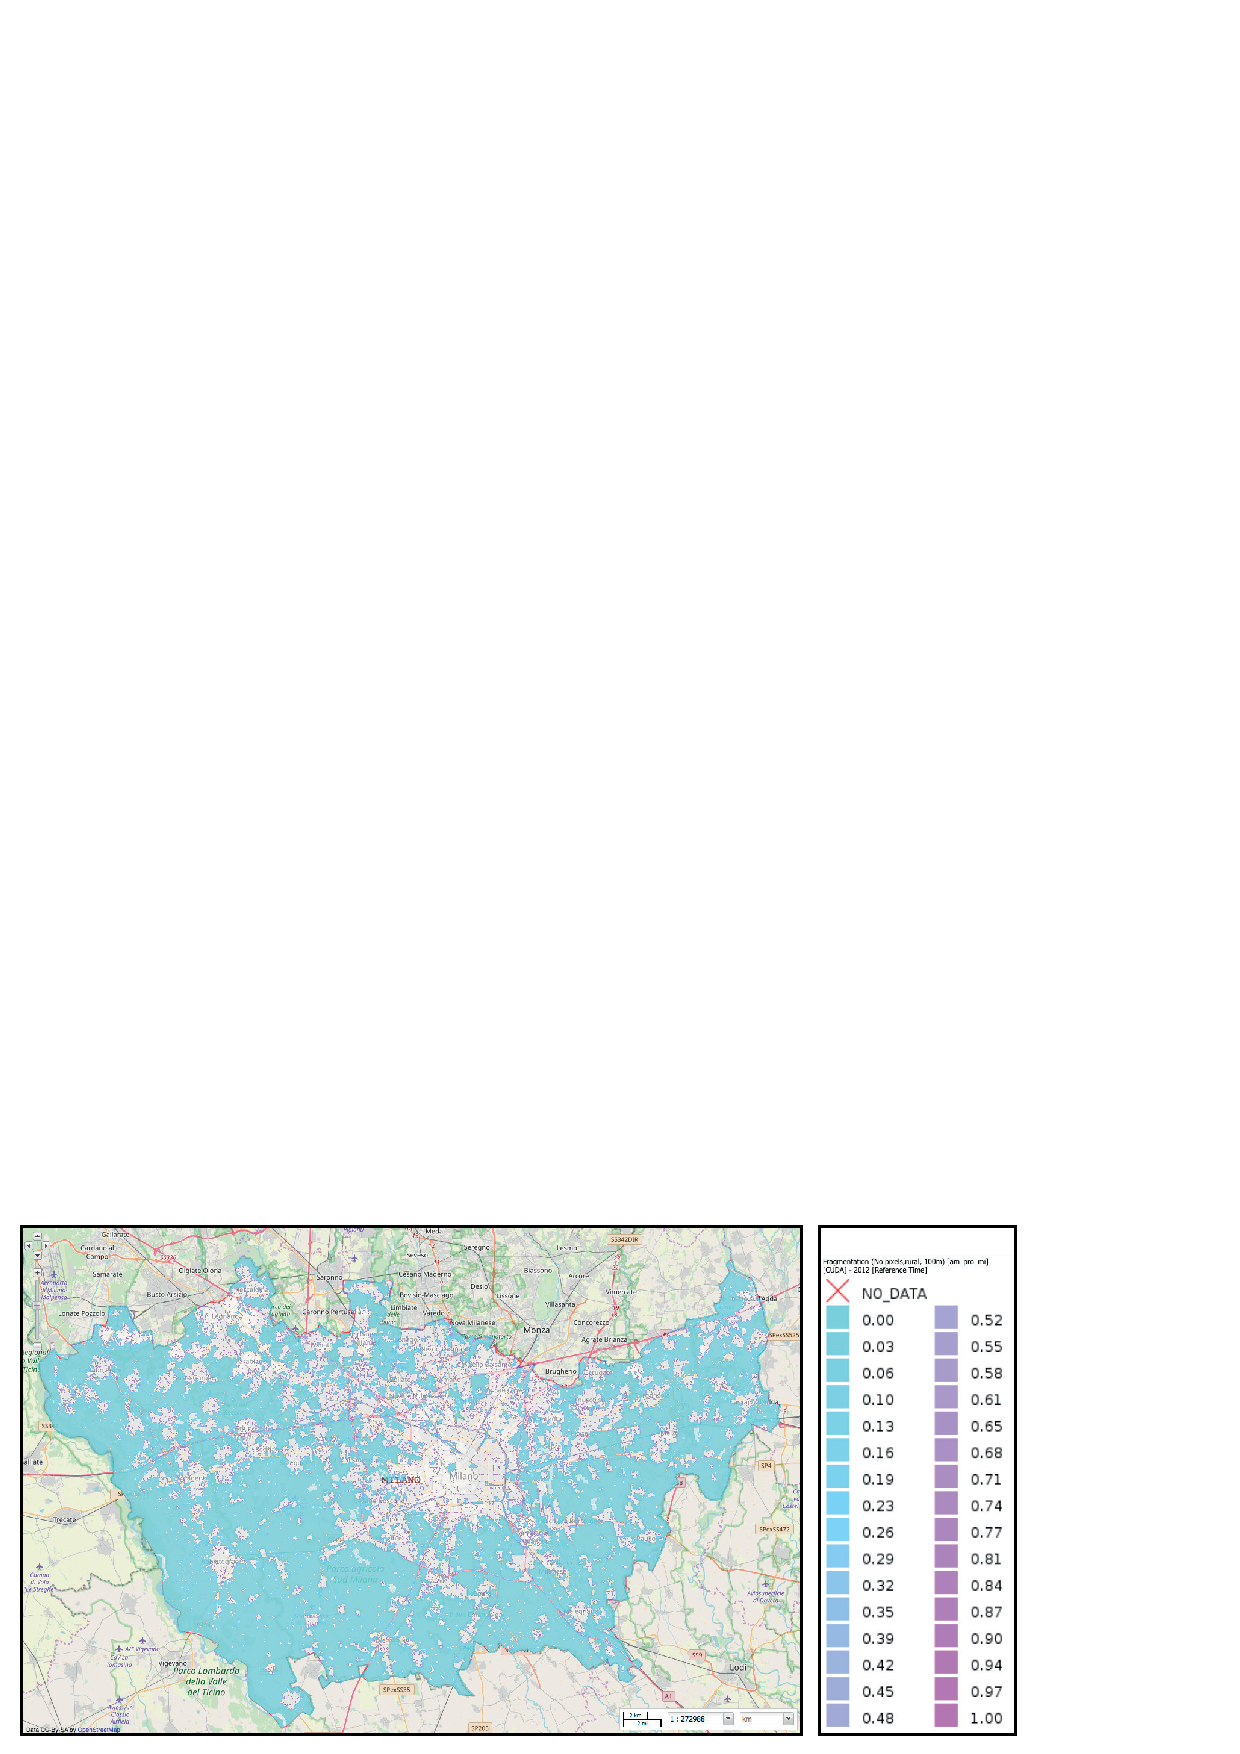
\includegraphics[width=450pt]{06_caso_provinciale.pdf}}
    \caption{ Map of rural fragmentation calculated in the province of Milan on 2012. } \label{fig:casePROV}
\end{figure}


\subsubsection{ Planning at the municipal level (PUC) }
\label{sec:caseCOM}

The municipal urbanization plan (PUC) is a tool for the management of the Italian municipal territory, which consists of cartographic and technical documents along with regulations for the management of urban and territorial transformations within the municipality.
The PUC stems from the old well known General Regulatory Plan (PRG established by Italian law 1150/1942); it is produced by urban planners assisted by experts from other fields (e.g. environmental scientists, pedologists, geologists, and lawyers).
Although the PUC has no duration limitations, it is periodically reviewed and has a long series of requirements, such as: (i) the identification and discipline of land uses; (ii) the subdivision of the territory into zones with different and complementary uses; (iii) the protection and enhancement of natural, landscape, and historical-cultural heritage. 
Moreover, since the PUC is the planning document closer to operational urban activities, it is important for Soil Monitor to be used at the municipal scale, where it enables (i) to analyse of a set of indicators of urban sprawl and of urban development, (ii) to support municipalities in having geospatial information useful for fulfilling the PUC requirements.

In the following it is shown the value of Soil Monitor in two different domains: (i) in quantification and analysis of land take dynamics and (ii) in municipality planning support. 

The study of quantification and analysis of land take dynamics at municipality level is presented in Figure \ref{fig:caseCOM_urbDev}, where a set of indicators for all the municipalities of the province of Napoli are reported for the quantitative analysis.
The statistics on \textit{Largest Class Patch Index} (LCPI) , \textit{Residual Mean Patch Surface} (RMPS) and \textit{Edge Density} (ED) metrics highlight a very large variation between the municipalities (Figure \ref{fig:caseCOM_urbDev}a).
More specifically, Casavatore shows a strong monocentric urban development with the highest LCPI value (LCPI: 99.98), while Monte di Procida has the most pronounced
polycentric nature with many small urban nuclei (RMPS: 1.18).
An analysis on edge density --- which is a good proxy of urban dispersion (e.g. \citealp{SCHWARZ2010}) --- shows that the rural mountain settlement of Agerola has the highest urban dispersion (ED: 1174) while the almost fully urbanized area of Casavatore shows the lowest urban dispersion trend (ED: 74).
Therefore, it is evident that these data requires further integration with other indexes such as the fraction of urbanized area and the population.
In Figure \ref{fig:caseCOM_urbDev}b we report a diagram quantifying ED for the municipalities of Napoli's province.
There are over 22 municipalities with a very high (>600) edge density and many of them refer to summer-based touristic sites in hilly and mountain sites (Agerola, Serra Fontana, Annacapri, Massalubrense, Vico Equense, Barano d'Ischia, Capri, Forio, Piano di Sorrento, etc.).
While the municipalities with the lower edge density (Casavatore, Arzano, Cardito, Melito di Napoli Portici) are not rural sites but rather strongly urbanized cities with very minimal and concentrated rural areas (thus low ED metric).

\begin{figure}
    \centerline{
        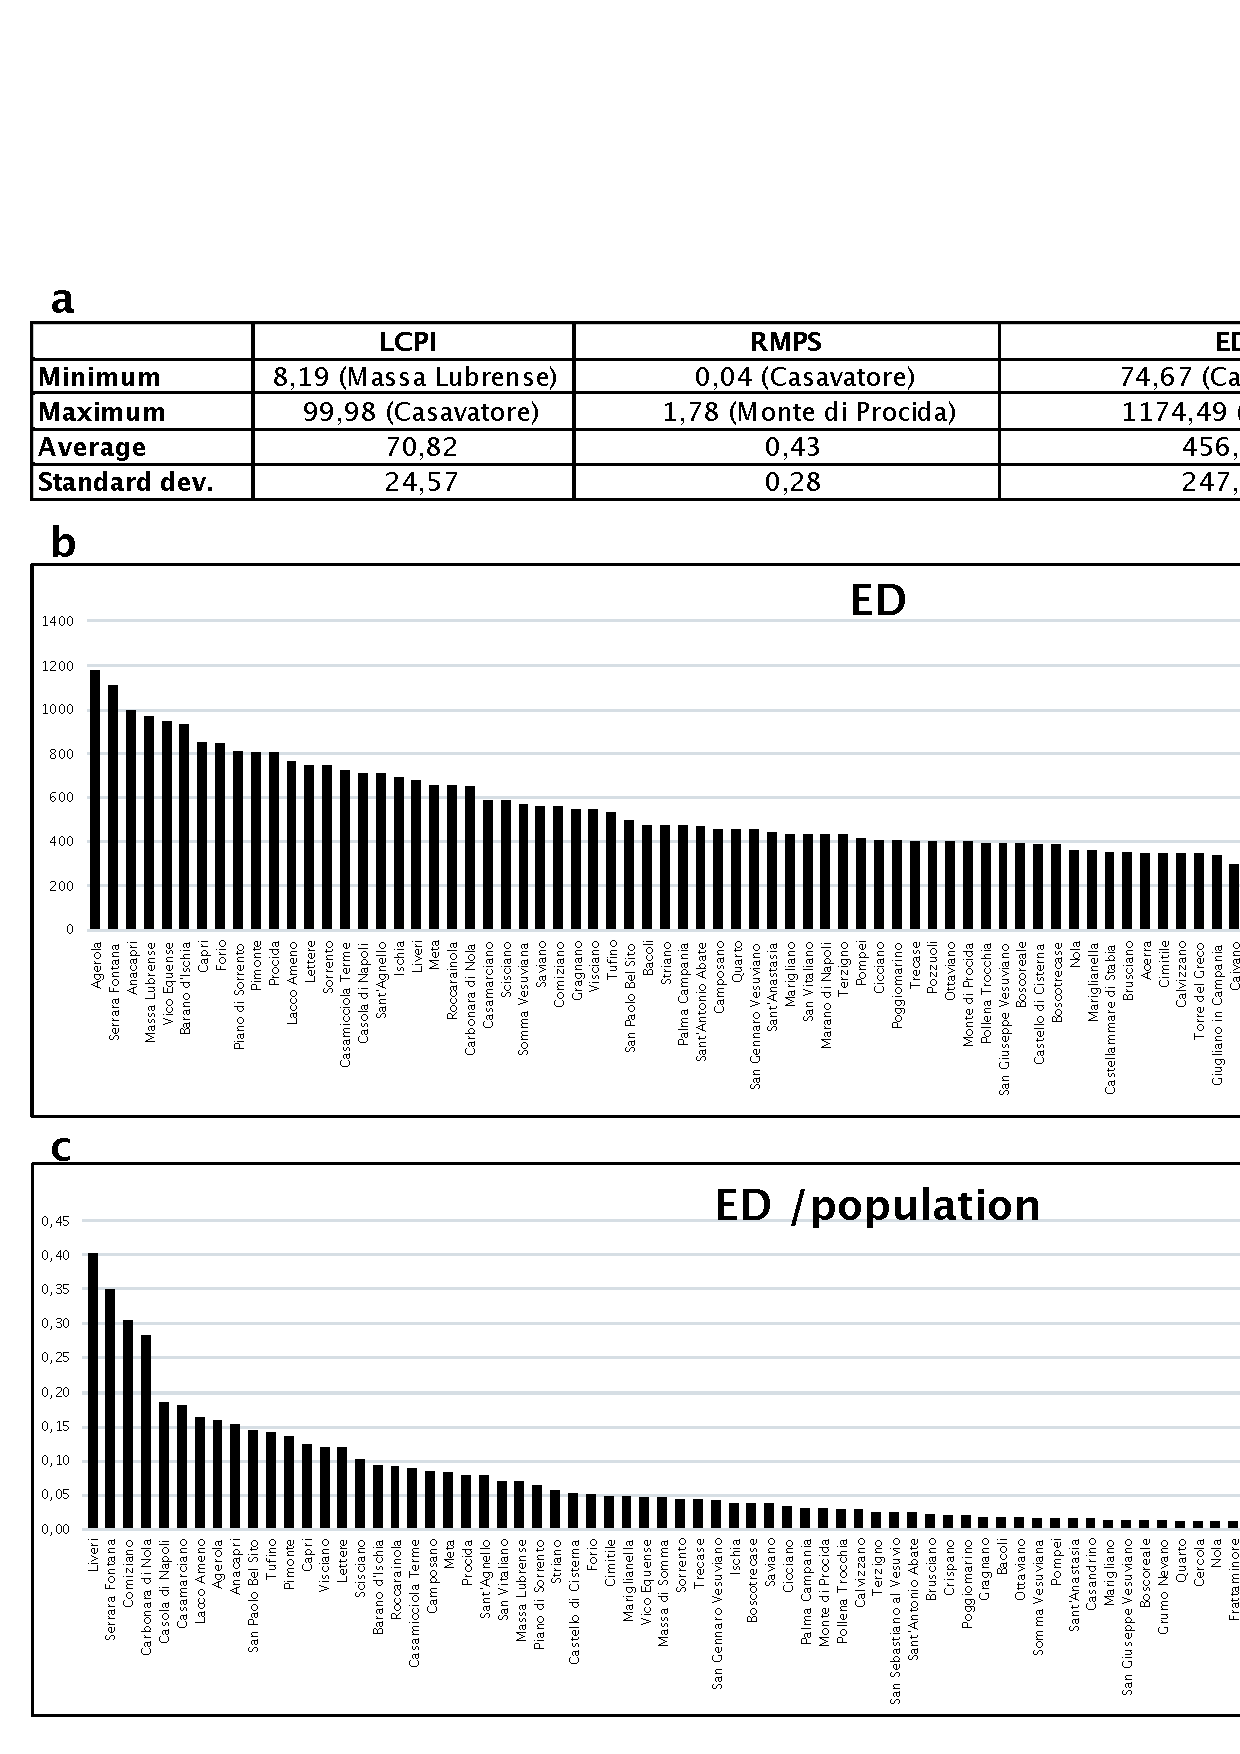
\includegraphics[width=450pt]{08_caso_comunale_tabella_grafici.pdf}
    }
    \caption{Quantitative analysis of the urban development of all municipalities within the province on Napoli (year 2012).
             (a) Summary statistics of metrics LCPI, RMPS and ED.
             (b) Edge density bar plot.
             (c) Bar plot of the ratio between edge density and population size.
             (LCPI: Largest Class Patch Index; 
             RMPS: Residual Mean Patch Surface; 
             ED: Edge Density)
            }
    \label{fig:caseCOM_urbDev}
\end{figure}

A more detailed analysis was then performed on the ratio between edge density and population size to highlight municipalities having a strong urban dispersion despite low population (Figure \ref{fig:caseCOM_urbDev}c).
This analysis points out that many small municipalities (e.g. Liveri, Comiziano, Carbonara di Nola,Casola di Napoli) --- well immerse in the rural environment and not having a touristic value --- show unexpected high ED/population values thus depicting a strong aggression of rural areas despite the very low population pressure.
From all analysis above it is evident the high explication value of the above indexes to better understand the urban development and, even more importantly, the impact of land take at municipality level.

In addition to the analysis of the land take dynamics given above, an analysis to support urban planning at the municipality level using Soil Monitor is provided in the following (Figure \ref{fig:caseCOM_Ercolano}).
The city of Ercolano is located between the Vesuvius volcano and the Tyrrhenian Sea, has a high population density, and is devoted to tourism owing to historical sites and spot of high-quality agriculture (e.g. wine, fruit trees, and flowers). 
Therefore, the user can get a quantification of the evolutive trajectories that led to specific land use and land cover states. 
In the example shown in Figure \ref{fig:caseCOM_Ercolano}(a, b), the amount and the geolocation of the consumption exerted by artificial surfaces is clear, above all, regarding vineyards, fruit trees, and olive orchards. 
This interpretation about the LULC evolution is accompanied by the recognition that part of the land take was very close (if not inside) to the protected areas (Figure \ref{fig:caseCOM_Ercolano}d) of the Vesuvius's slopes, thereby confirming the very high pressure of urbanization not well managed by local authorities. 
Accordingly, the model of urban development was computed in the same municipality of Ercolano against other most populated cities in the Napoli province. 
Figure \ref{fig:caseCOM_Ercolano}(c) shows the population size and density (the left side of the table) and the indicators of model of urban development (LCPI, RMPS, and ED on the right side of the table), depicting the main urban trends in the Napoli province.
These results are limited examples of the awareness building that can be achieved using Soil Monitor, which in turn profitably supports the definition and implementation of plans at the municipality scale (PUC in Italy).
This finding becomes much more important considering Soil Monitor is operational over the entire Italian territory with more than eight thousand municipalities.

\begin{figure}[t] % FIGURE 06
    \centerline{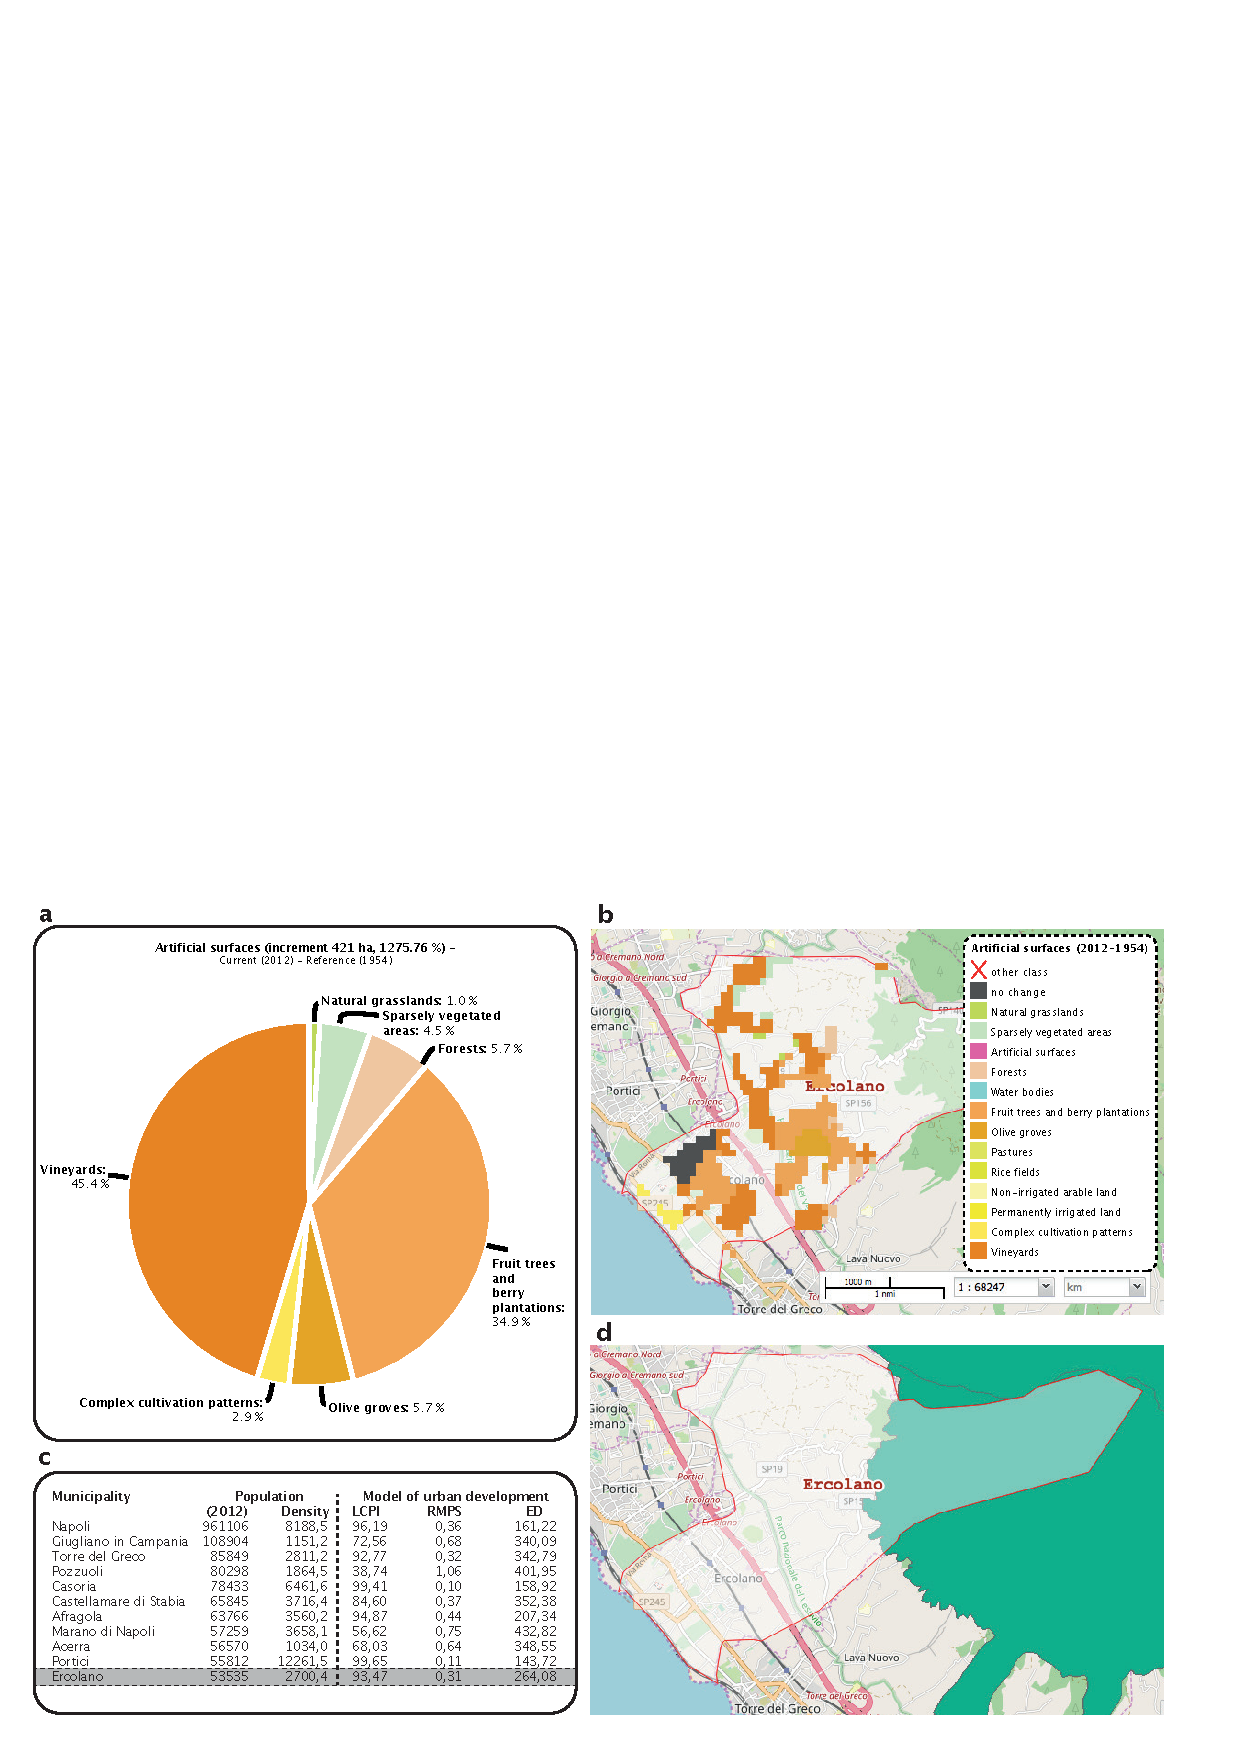
\includegraphics[width=450pt]{07_caso_comunale.pdf}}
    \caption{ Soil Monitor supports the analysis at the level of the municipal urbanization plan (PUC) in Ercolano municipality.
              (a) Pie chart of the LULC changes in Ercolano towards artificial surfaces in 2012 from all other classes in 1954.
              (b) Image map of the changes in Ercolano depicted in (a).
              (c) Data and metrics supporting the quantitative analysis at the municipality level.
              (d) The Ercolano RoI in contrast with the landscape constraints given by Vesusius national park (dark green). }
    \label{fig:caseCOM_Ercolano}
\end{figure}

\subsection{Final discussion}
Soil Monitor is designed to address the accountancy of soil sealing through different indicators providing operational support to urban planners, decision makers and multi stakeholders involved in landscape planning and interested in evaluating the impact of soil sealing. 
This specific contribution required a different approach, the result of which is the Soil Monitor geospatial cyber-infrastructure. 
A set of indicators can be calculated in real-time using either Italian administrative levels (NUTS2, NUTS3, and LAU2) or user-drawn Regions of Interest (RoI). 
Moreover, Soil Monitor uses high resolution layers produced every year by ISPRA (Italian Institute for Environmental Protection and Research) since 2015 for drawing up their yearly soil sealing report in Italy. 
Thus, owing to the high-performance computing embedded in its cyber-infrastructure, Soil Monitor enables real-time geospatial processing while preserving a high spatial detail of the analysis over large areas (till LAU2, but it can scale according to available hardware).
This combination of features has an intrinsic vast potential for being used in operational spatial planning as testified by the results presented in this work. 

Despite the huge endeavour spent on the logic tier to have GPU computing on board of Soil Monitor, the platform shows some important limitations caused by constraints in the data.
First, one main limitation is the lack of soil information underpinning the analysis, % in Soil Monitor, 
such as the lack of different qualities of soils and their spatial distribution in the scenario analysis.
But unfortunately there not exists a detailed and homogeneous soil map for whole Italy.
To smoothly mitigate the fundamental shortcoming of not having soil information and to help discriminating between the different land qualities vulnerable to land take, Soil Monitor shows (via WMS protocol) soil grids at 250m spatial resolution produced by ISRIC.
Attention should be drawn to the low accuracy of this grids with respect to the scale and the detail of the land take and soil sealing analysis available in Soil Monitor.
Second, the base data (i.e. imperviousness layers) used in the analysis can have inconsistencies that Soil Monitor highlights.
It is possible to get artefacts in results %produced by Soil Monitor 
because of possible issues in the production of the data (performed by ISPRA or Copernicus), artefacts that are not caused by Soil Monitor procedures. %that does not involve Soil Monitor.
These issues can be caused by a misclassification of features over time with impervious covers unrealistically fluctuating over time (e.g. up and down from 0\% to 100\%) or by not detecting sealed surfaces mostly in less urbanized or rural areas.
Even though some these artefacts leads to an evident underestimation of the land degradation process, they are sporadic.

In the presentation of the Java/JCUDA/CUDA pipeline embedded in Soil Monitor (section \ref{sec:logicTier}) 
it was shown that the JCUDA layer performs calls to the CUDA kernels compiled in PTX files to address the calculation of a soil sealing metric.
The proposed pipeline is an absolute technological novelty in the implementation of geospatial decision support systems based on WebGIS and it enables the deployment of a fast geoprocessing engine capable to support a multi-user and multi-tasking web application.
To author knowledge, the
integration of high performance computing by means of the CUDA framework within web based geospatial cyber-infrastructures is absolutely new.
This is an important result that must be emphasized here not only for the technological advancement itself, but because this technology is firstly applied to soil sealing and land degradation issues and because it changes the way in which different stakeholders (citizens, technicians, professionals, policy makers, etc.) can get informed about and measure soil sealing with agreed, validated and standard methods.

\section{Conclusions}
Soil sealing is an important form of land degradation worldwide and its mitigation implemented through best practices in spatial land planning is a very virtuous goal.
Undoubtedly, the high quantity of information that is increasingly accessible for instance through satellites and drones to tackle agricultural, forestry, environmental and spatial planning issues is simply not sufficient to face the complexity of soil sealing mitigation.
It is necessary to raise awareness in different sectors (policy, research and public) and to fund research and trans-disciplinary studies aiming to mitigate the phenomenon.
Authors call attention to the current gap in the availability of factual tools that tackle soil sealing and enable quantitative analysis, awareness building and decision making. 
The objective of this work coped with the development of a new technological solution based on geospatial cyber-infrastructures to provide an operational tool capable to study, challenge and mitigate soil sealing at different planning and spatial scales.
We demonstrated that tools such as Soil Monitor --- which is freely accessible via an internet browser without the need to install any application or plugin on the local computer --- have significant potential to fill the current gap.
The combination of WebGIS with GPU computing which runs on-the-fly geospatial processing puts Soil Monitor at the fringe of research and development. 
This kind of technology demonstrated promising capability to quantitatively measure soil sealing and to give a contribution to mitigate the %continual 
phenomenon worldwide, considering the high transferability of the proposed cyber-infrastructure.
Nevertheless, the proposed platform still remains a prototype from research that anyway can be used in whole Italy. 
Subsequently, it can be seen as a democratic tool for creating reports that can catch the evolution of land use trajectories and connected land degradation interpretations about the ongoing of land degradation processes.

\section*{ORCID}
Giuliano Langella \href{https://orcid.org/0000-0001-7210-0906}{ {\orcidicon{0000-0001-7210-0906}}\hspace{1.0mm} orcid.org/0000-0001-7210-0906}

\bibliography{SMapp}

\end{document}